% !Mode:: "TeX:UTF-8"
% !TEX program  = xelatex
%\documentclass{cumcmthesis}
\documentclass[withoutpreface,bwprint]{cumcmthesis} %去掉封面与编号页,电子版提交的时候使用。
\usepackage{etoolbox}
\BeforeBeginEnvironment{tabular}{\zihao{-5}}
\usepackage{cite}
\usepackage[numbers,sort&compress]{natbib}
\usepackage[framemethod=TikZ]{mdframed}
\usepackage{url}   % 网页链接
\usepackage{subcaption} % 子标题
\usepackage{bm} %公式加粗
\title{基于转动定理的半圆形薄片运动建模}
\tihao{A}
\baominghao{4321}
\schoolname{华中科技大学}
\membera{ }
\memberb{ }
\memberc{ }
\supervisor{ }
\yearinput{2020}
\monthinput{08}
\dayinput{22}




\begin{document}
	
	\maketitle
	\begin{center}
	姓名:\underline{ 郑文斌 } 班级:\underline{ 光电1902 } 学号:\underline{ U201913935}
\end{center}

	\begin{abstract}
		 为解决问题一,本文首先对半圆形薄片系统建立\textbf{受力方程、力矩方程、几何方程},通过数值方法求解方程组得到了施加拉力后半圆形薄片的倾角\bm{$\theta = 0.1564rad$}.
		 
		 
		 对于问题二,半圆形薄片的运动为周期运动,可分解为竖直方向运动和转动两个方面。由于问题一求解的$\theta$值较小,\textbf{忽略竖直方向运动}。以问题一求解结果为初始角度,对问题二基于转动定理建立\textbf{转动微分方程},通过几何关系建立变量之间的约束,利用ode45求解微分方程,求解得到的\textbf{短期}内角度随时间变化的曲线为\textbf{周期约为\bm{$0.3s$}的余弦函数曲线}。同时,本文对\bm{$\theta \approx 0$}的极限情况,作了近似分析,求出其\textbf{近似周期解析解},作出了周期与劲度系数、半径、质量的关系。
		
		对于问题三,利用与前两问的相似性,添加了两个角度未知量,对应地建立第一小问的方程组,求得\bm{$\theta = 0.1562rad$};建立第二小问的\textbf{微分代数方程},利用ode15s或者迭代法+ode45求解。同时,本文也对此模型分析了$\theta \approx 0$的极限情况。
		
		由于问题一和问题3-1求解的倾角较小,模型忽略竖直方向运动,简化了方程和求解过程,但也同时造成\textbf{长期}演化后,出现\textbf{角度衰减}的现象,即能量不守恒的假象,和实际情况不符。针对此问题,在模型的推广中,本文对问题的实际情况做了分析,\textbf{综合考虑转动和竖直方向运动},对竖直方向运动作出了简化的模型,描述了竖直运动的周期。半圆形薄片的真实运动周期应该介于竖直运动周期和转动周期之间。
		
		\keywords{受力平衡 \quad 转动定理  \quad 微分代数方程\quad  周期运动}
	\end{abstract}
	
	%目录  2019 明确不要目录,我觉得这个规定太好了
	\tableofcontents
	
	\newpage
	
	\section{问题重述}
	一个质量为5千克的均质半圆形薄片由两根相同的轻质硬弹簧通过半圆形薄片的直径两端悬挂在一根水平光滑横梁上。弹簧与横梁的接触点没有固定,弹簧可在横梁上自由滑动。
	薄片的半径为0.3米, 弹簧的倔强系数为500牛/米。今在直径的B端施加一个50牛的向下的拉力。试回答如下问题:
	
	1.	在系统平衡后,请给出半圆形薄片的倾角θ是多少度?
	
	2.	在撤去拉力后,给出100秒内薄片倾角的变化情况。
	
	3.	假设两个弹簧的原始长度是0.5米,弹簧上端固定在横梁上,弹簧间距是0.6米。在B端施加一个向下的50牛拉力后,试解答此情形下的1-2问。
	
	
	\section{问题分析}
	\subsection{问题一分析}
	未施加外力前,两弹簧竖直;施加外力后,由于杆光滑,无摩擦力,两弹簧保持竖直。列出受力平衡方程,以圆心为参考点,有力矩的平衡关系,再通过几何关系可以建立方程组,即可求解$\theta$角。
	
	\subsection{问题二分析}
	由于能量守恒,半圆形薄片一定做周期运动,其运动可分解为转动和竖直方向运动。
	
	释放外力后,由于$\theta$角较小,半圆形薄片近似绕过圆心且垂直于转动于薄片的直线作定轴转动,可以由转动定理建立转动微分方程,并由几何关系添加相关自变量之间的约束,通过求解微分方程求解角度时间演化关系。
	
	\subsection{问题三分析}
	对于问题三,其与问题一和问题二具有相似性。添加若干相关自变量,同样建立方程组和微分方程组及约束,求解过程同理。
	
	\section{模型假设}
	\begin{itemize}
		\item 外力F较小,导致$\theta$角较小时,半圆形薄片竖直方向的运动可忽略,近似绕过圆心且垂直于转动于薄片的直线作定轴转动	;
		\item  系统无摩擦力,能量守恒;	
	\end{itemize}
	
	\section{符号说明}
	% Table generated by Excel2LaTeX from sheet 'Sheet1'
	\begin{table}[H]
		\centering
		\begin{tabularx}{\textwidth}{@{}c *2{>{\centering\arraybackslash}X}@{}}
			\toprule[1.5pt]
			符号    & 说明    & 量纲 \\
			\midrule
			$\theta$ & 题中所求角度 & $rad$ \\
			$\omega,\theta^{\prime}$ & 角速度   & $rad/s$ \\
			$\alpha,\theta^{\prime \prime}$ & 角加速度  & $rad/s^2$ \\
			$J     $	 & 半圆形薄片的转动惯量 &$ kg·m^² $\\
			$M     $	& 合力矩   & 牛/米 \\
			$x_1    $	& 左弹簧的形变 & 米 \\
			$x_2    $	& 右弹簧的形变 & 米 \\
			$\theta_1$	 & 左弹簧与水平线的夹角 & $rad$ \\
			$\theta_2$	 & 右弹簧与水平线的夹角 & $rad$ \\
			$k     $	& 弹簧的倔强系数 & 牛/米 \\
			$g     $	& 重力加速度 & $m/s^2$ \\
			$r     $	& 半圆形薄片的半径 & 米 \\
			$F     $	& 施加的外力 & 牛 \\
			$m     $	& 半圆形薄片的质量 & 千克 \\
			$\Delta x$	 & 半圆形薄片的重心到圆心的距离 & 米 \\
			$L     $	& 两弹簧间距 & 米 \\
			$l     $	& 弹簧原长  & 米 \\
				$T    $	& 运动周期  & 秒 \\
			\bottomrule[1.5pt]
		\end{tabularx}%
		\label{tab:addlabel}%
	\end{table}%
	
	
	\section{问题一模型}
	\subsection{模型的建立}
	弹簧与横梁的接触点没有固定,弹簧可在横梁上自由滑动。假设施加外力F后弹簧与横梁不垂直,在弹簧拉力的水平分量的作用下,弹簧不平衡而发生运动,直至垂直。所以弹簧与横梁保持垂直。
	
	施加外力F后,半圆形薄片发生旋转,选取其圆心作为旋转参考点,作出受力图如图\ref{问题1受力示意图}
	 \begin{figure}[H]
		\centering
		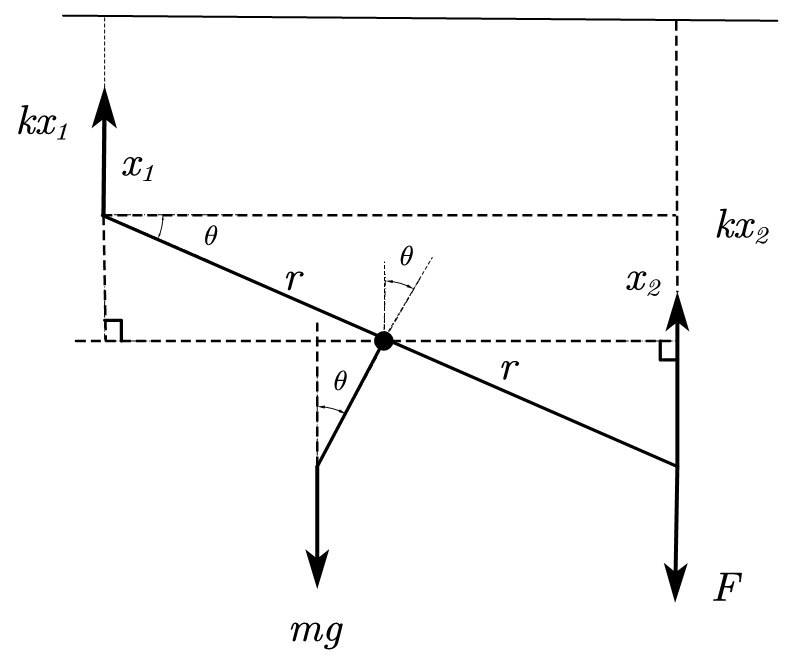
\includegraphics[width=0.7\textwidth]{问题1受力示意图}
		\caption{问题1受力示意图}
		\label{问题1受力示意图}
	\end{figure}
	半圆重心到圆心的距离$\Delta x $为
	\begin{equation}
		\Delta x = \frac{4 r}{3 \pi} 
		\label{zx}
	\end{equation}	
	设左弹簧形变量为$x_1$,右弹簧形变量为$x_2$,由受力平衡,可得:
	\begin{equation}
	k x_{1}+k x_{2}=F+m g
	\label{slph1}
	\end{equation}	
	由力矩平衡,得:
	\begin{equation}
	k x_{2} r \cos \theta+m g \Delta x \sin \theta=k x_{1} r \cos \theta+F r \cos \theta
	\label{ljph1}
	\end{equation}
	因为两弹簧竖直,又可得几何关系:
	\begin{equation}
	\sin \theta=\frac{x_{2}-x_{1}}{2 r} 
	\label{jhgx1}
	\end{equation}
	联立式(\ref{zx})(\ref{slph1})(\ref{ljph1})(\ref{jhgx1})可得:
	\begin{equation}
	\left\{\begin{array}{l}
	k x_{2} r \cos \theta+m g \frac{4 r}{3\pi} \sin \theta=k x_{1} r \cos \theta+F r \cos \theta\\
	\sin \theta=\frac{x_{2}-x_{1}}{2 r} \\
	k x_{1}+k x_{2}=F+m g
	\end{array}\right.
	\label{q1}
	\end{equation}
	
	
	
	\subsection{模型的求解}
	方程组(\ref{q1})无解析解,但可使用数值法求解,使用fsolve函数,设置$x_1,x_2,\theta$的初值为$0,0,0$,迭代求解,解得$\theta=0.1564rad,x_1=0.0523 (m),x_2=0.1457(m)$.

	
	\section{问题二模型}
	\subsection{模型的建立}
	规定半圆形薄片向右倾斜$\theta$为正,斜$\theta$为负,作出受力图,如图\ref{问题2受力示意图}。
	 \begin{figure}[H]
		\centering
		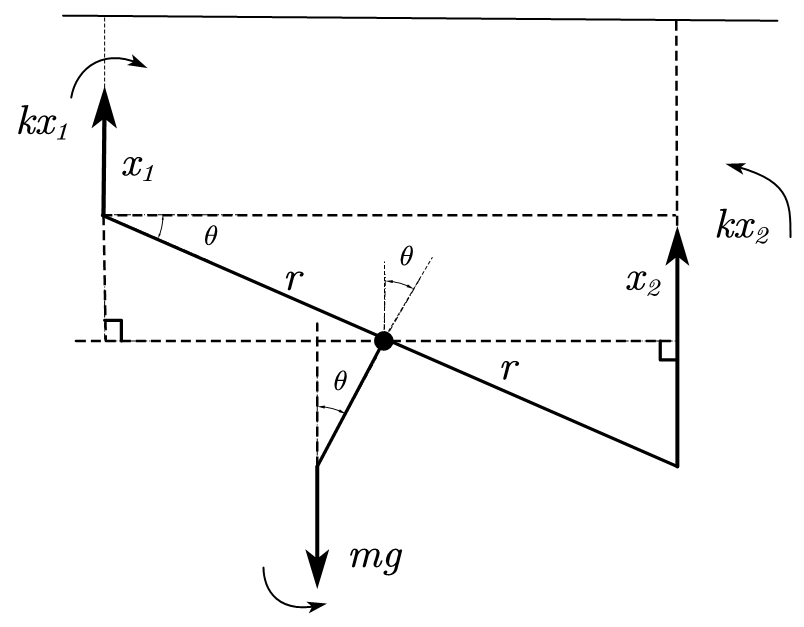
\includegraphics[width=0.7\textwidth]{问题2受力示意图}
		\caption{问题2受力示意图}
		\label{问题2受力示意图}
	\end{figure}
	
	由于问题一求解出的$\theta$角较小,半圆形薄片竖直方向的运动可忽略,近似绕过圆心且垂直于转动于薄片的直线作定轴转动。
	
	撤去外力F后,半圆形薄片在弹簧拉力的作用下向平衡位置旋转。撤去外力F的一瞬间,角速度为0,角加速度为负的最大值,半圆形薄片运动到平衡位置时,角速度为负的最大值,角加速度为0,$\theta$开始变为负值。设问题一中求得的$\theta=\theta_0$,由于无摩擦力,能量守恒,半圆形薄片最终能运动到对称的位置,此时$\theta=-\theta_0$,之后重复上述过程,由此可知,半圆形薄片做类似简谐运动。
	
	由转动定理\upcite{liFeiDingZhouZhuanDongZhiTuiGunDongZhouChengEDingDongZaiHeDeYanJiu2016,liGangDanXingFuZaXiTongZaiChongLiChangZhongDeDingDianZhuanDong1995,wangFeiWanZhengYingSheLiLunYuGangTiDingDianZhuanDongDeJiHeMiaoShu2009}:
	\begin{theorem}
		刚体在做定轴转动时,刚体的角加速度与它所受到的合外力矩成正比,与刚体的转动惯量成反比。
		\label{lem:example}
	\end{theorem}
	 
	\begin{equation}
	\left\{\begin{array}{l}
	M=J \alpha\\
	J=\frac{m r^2}{2}\\
	\alpha = \frac{d^{2} \theta}{d t^{2}} = \theta^{\prime \prime}
	\label{zddlq2}
	\end{array}\right.
	\end{equation}
	其中$J$为半圆形薄片的转动惯量,$\alpha$为角加速度。
	求出系统的合力矩$M$,代入式\ref{zddlq2},得力矩约束方程:
	\begin{equation}
	k\left(x_{1}-x_{2}\right) r \cos \theta-\frac{4 mg r}{3\pi} \sin \theta=\frac{mr^{2}}{2} \theta^{\prime \prime}
	\label{ljysfc}
	\end{equation}
	将几何约束方程式\ref{jhgx1}代入式\ref{ljysfc},消去$x_1,x_2$,可得以下初值问题:
	\begin{equation}\label{czq2}
	\left\{\begin{array}{l}
	\theta^{\prime \prime}=-\frac{8g}{3 \pi r} \sin \theta-\frac{4 k}{m} \sin \theta \cos \theta \\
	\theta(0)=\theta_{0} \quad \theta^{\prime}(0)=0
	\end{array}\right.
	\end{equation}
	\subsection{模型的求解:数值法}
	式(\ref{czq2}) 无解析解,但可以通过数值方法求解数值解。令$\theta^{\prime}=\omega$,$\omega$为角速度,将二阶导数转化为两个一阶导数,使用ode45求解初值问题(\ref{czq21}),
		\begin{equation}\label{czq21}
	\left\{\begin{array}{l}
	\theta^{\prime}=\omega\\
	\omega^{ \prime}=-\frac{8g}{3 \pi r} \sin \theta-\frac{4 k}{m} \sin \theta \cos \theta \\
	\theta(0)=\theta_{0} \quad \theta^{\prime}(0)=0
	\end{array}\right.
	\end{equation}
	设置$\theta,\omega$的初值分别为$\theta_0,0$,解得5s内角度$\theta$和角速度$\omega$随时间变化的关系如图\ref{模型1角度及角速度随时间的变化}.
		 \begin{figure}[H]
		\centering
		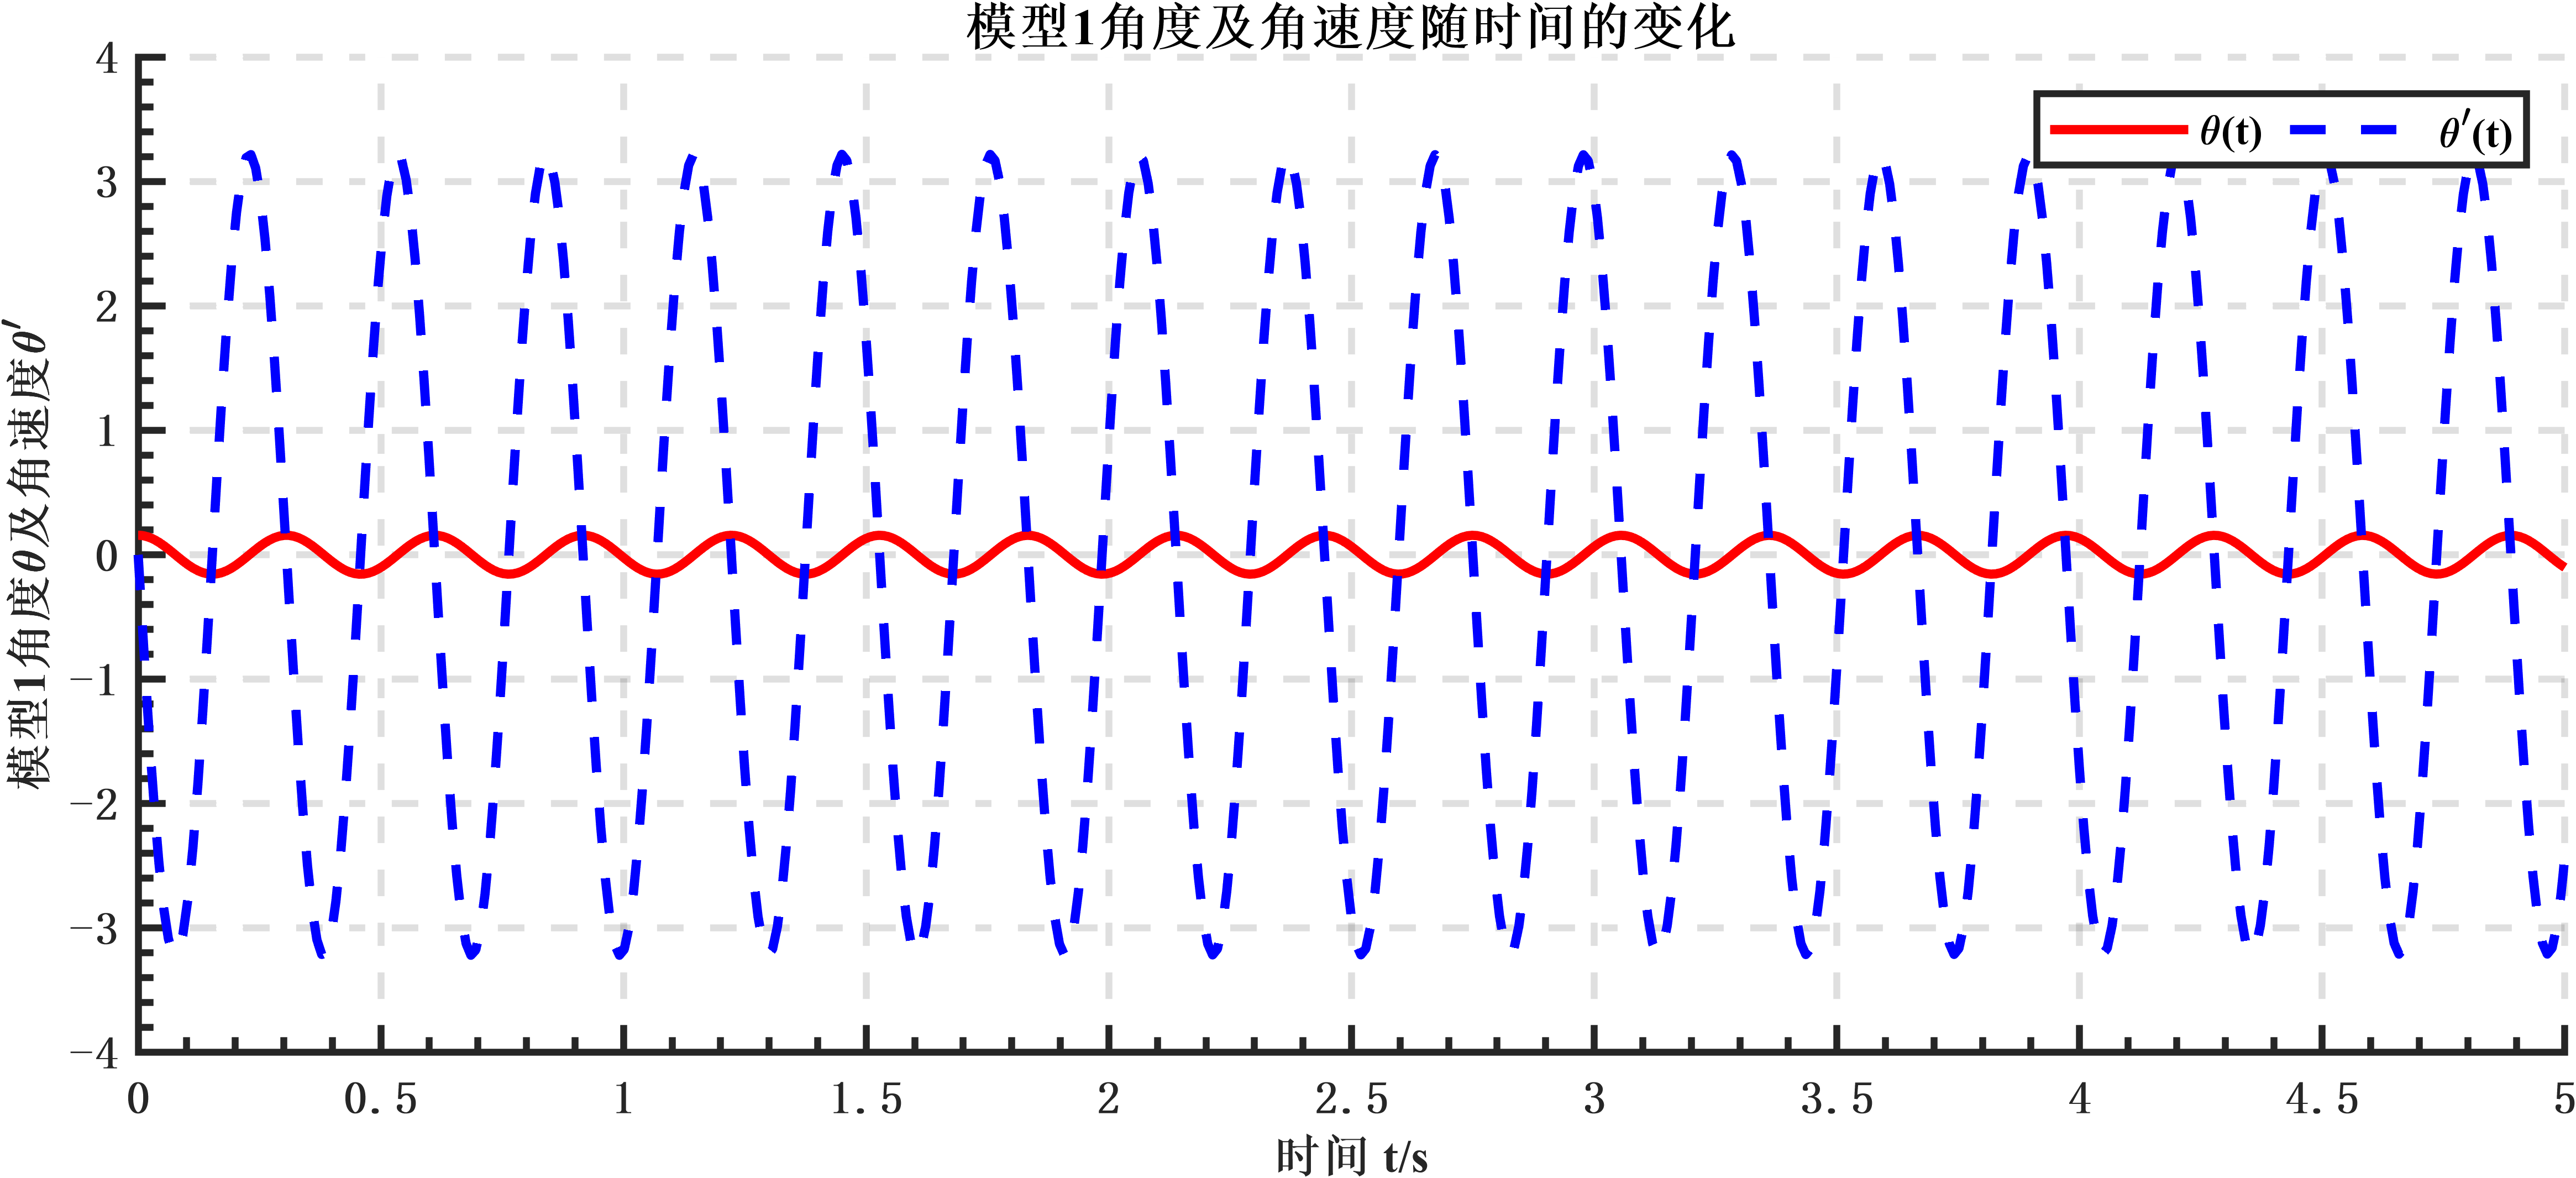
\includegraphics[width=0.85\textwidth]{模型1角度及角速度随时间的变化}
		\caption{模型1:角度及角速度随时间的变化}
		\label{模型1角度及角速度随时间的变化}
	\end{figure}
	角度与角速度的关系如图\ref{模型角度角速度角加速度相图}.
			 \begin{figure}[H]
		\centering
		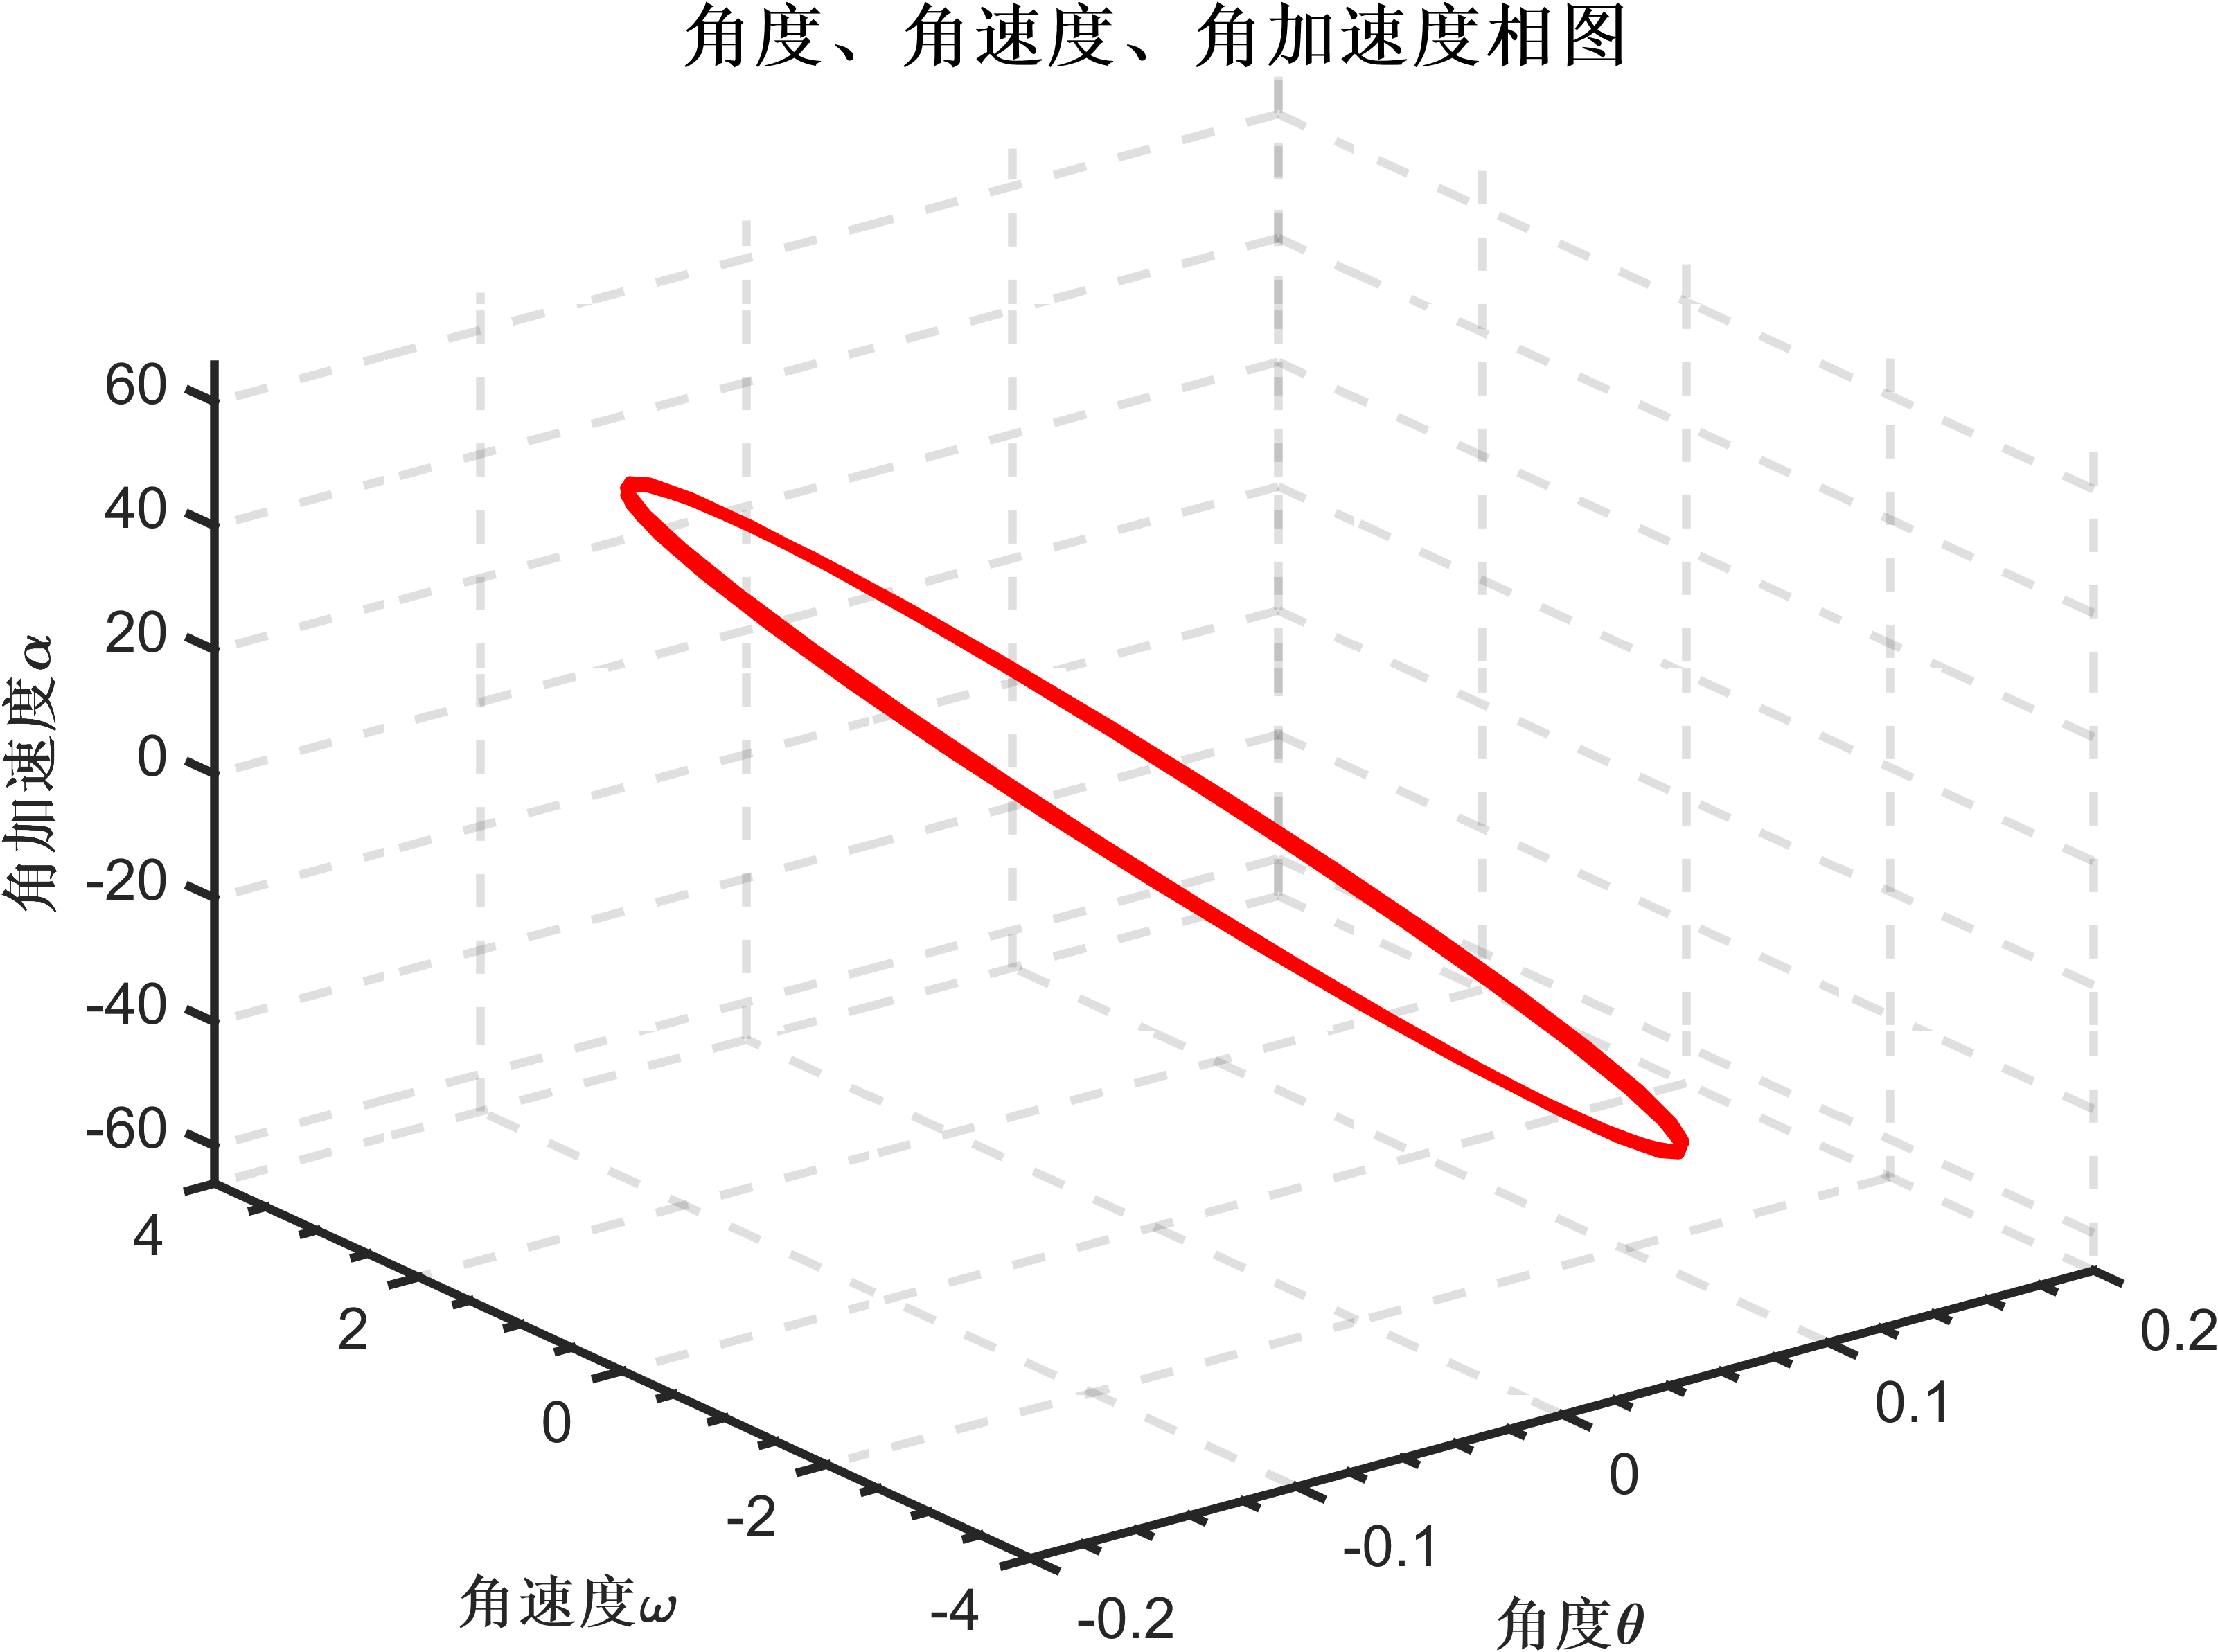
\includegraphics[width=0.6\textwidth]{模型1角度角速度角加速度相图}
		\caption{模型1:角度、角速度、角加速度相图}
		\label{模型角度角速度角加速度相图}
	\end{figure}
   由图\ref{模型1角度及角速度随时间的变化}计算运动的周期$T\approx 0.30s$
   
   以上是短期变化情况,作出长期情况下(1000s)角度与角速度的变化情况如图\ref{模型1角度及角速度随时间的变化1000s}.由图可知,在该模型方程的描述下,物体不是做的严格的简谐运动,半圆形薄片所能到达的最大$\theta$随着时间的增加而减小.由图\ref{模型1角度角速度角加速度相图1000s}中的相图可以得知,$\theta,\theta^{\prime},\theta^{\prime \prime}$都在向0靠近。$t \rightarrow  \inf $时,$\theta,\theta^{\prime},\theta^{\prime \prime} \rightarrow 0 $.
   
   图\ref{模型1角度及角速度随时间的变化1000s}和图\ref{模型1角度角速度角加速度相图1000s}说明系统能量在衰减,但是,由于系统能量守恒,不可能出现能量衰减的情况,也就是说,模型推导出的长期变化情况与实际不符。
   
   出现这种情况的原因在于,实际上半圆形薄片作的并不是定轴运动,参考点圆心的位置随着时间变化,而模型是基于定轴运动建立的,这就导致了能量不守恒的假象。在“模型的推广”一节,本文对实际情况进行了定性分析。
   			 \begin{figure}[H]
   	\centering
   	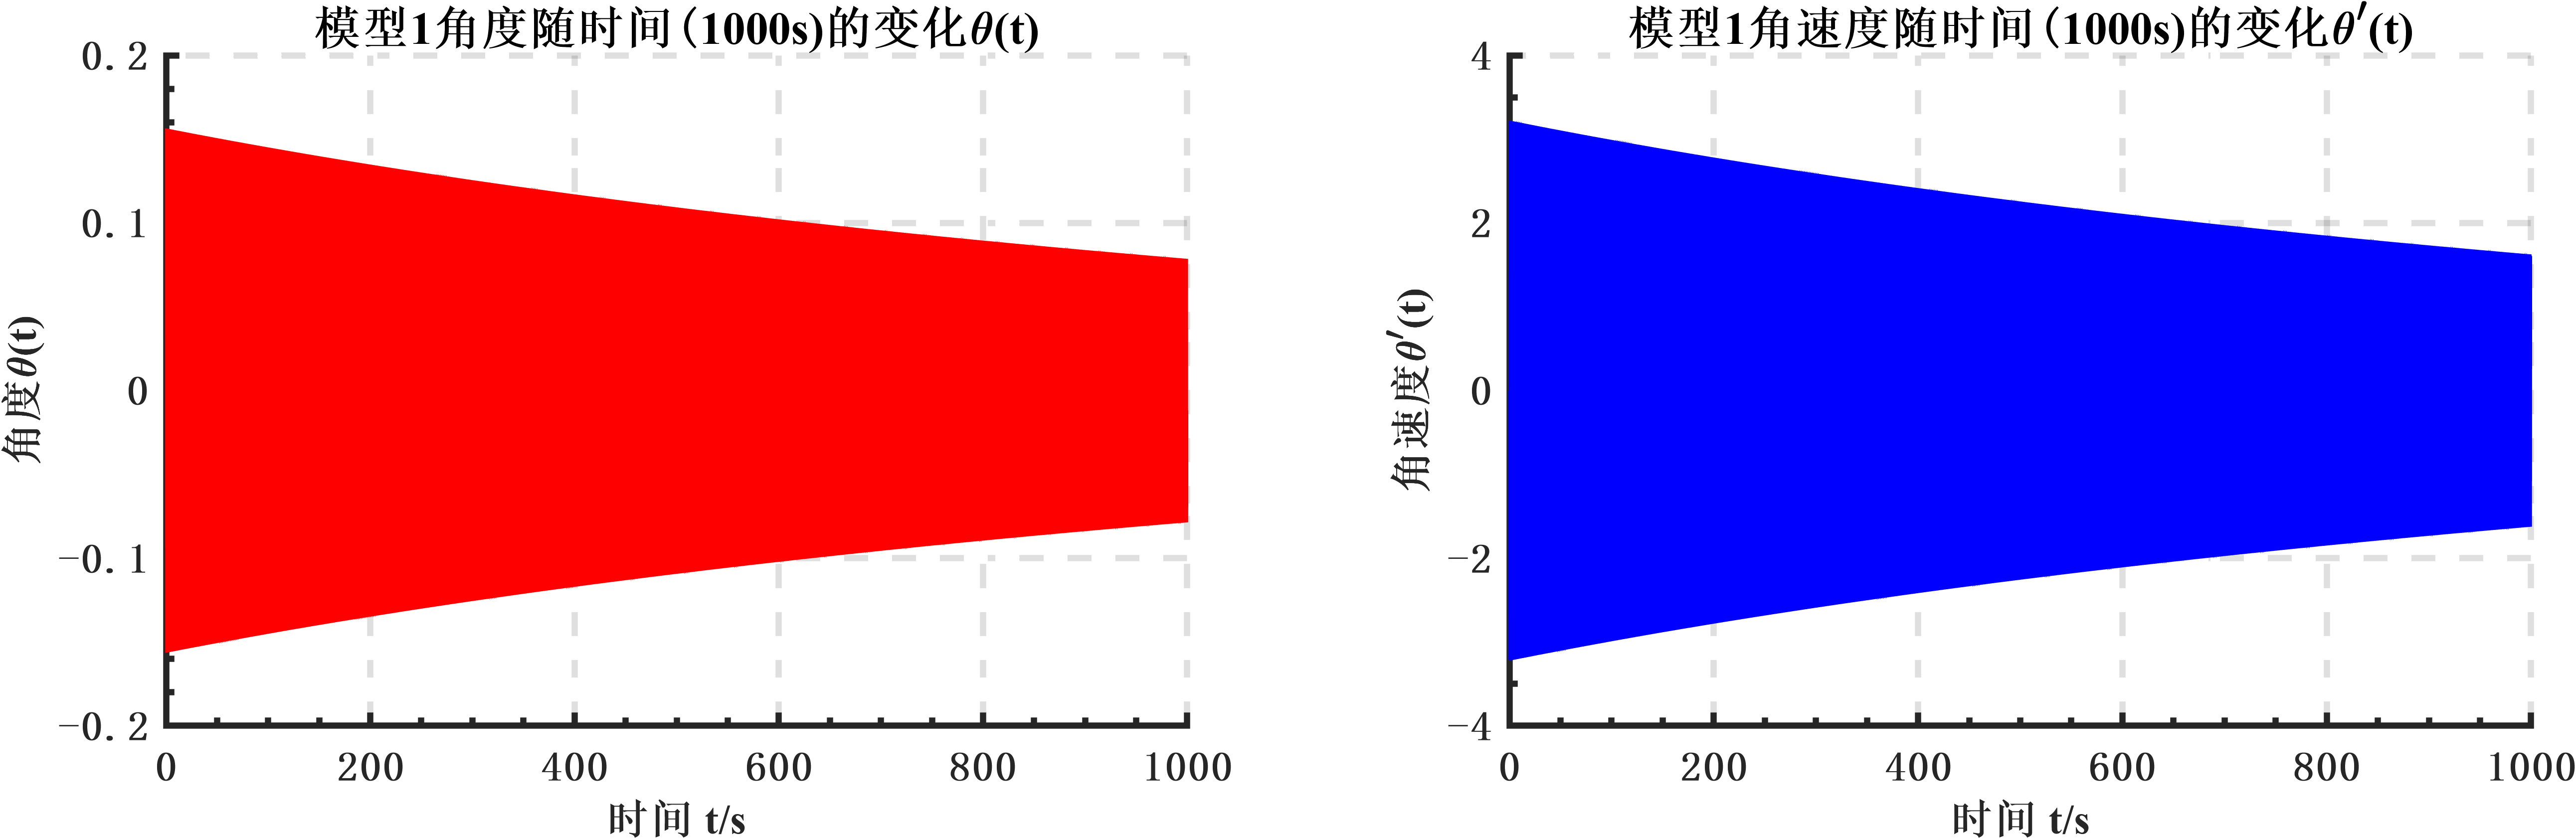
\includegraphics[width=0.9\textwidth]{模型1角度及角速度随时间的变化1000s}
   	\caption{模型1: 1000s内角度、角速度的变化}
   	\label{模型1角度及角速度随时间的变化1000s}
   \end{figure}

 	\begin{figure}[H]
	\centering
	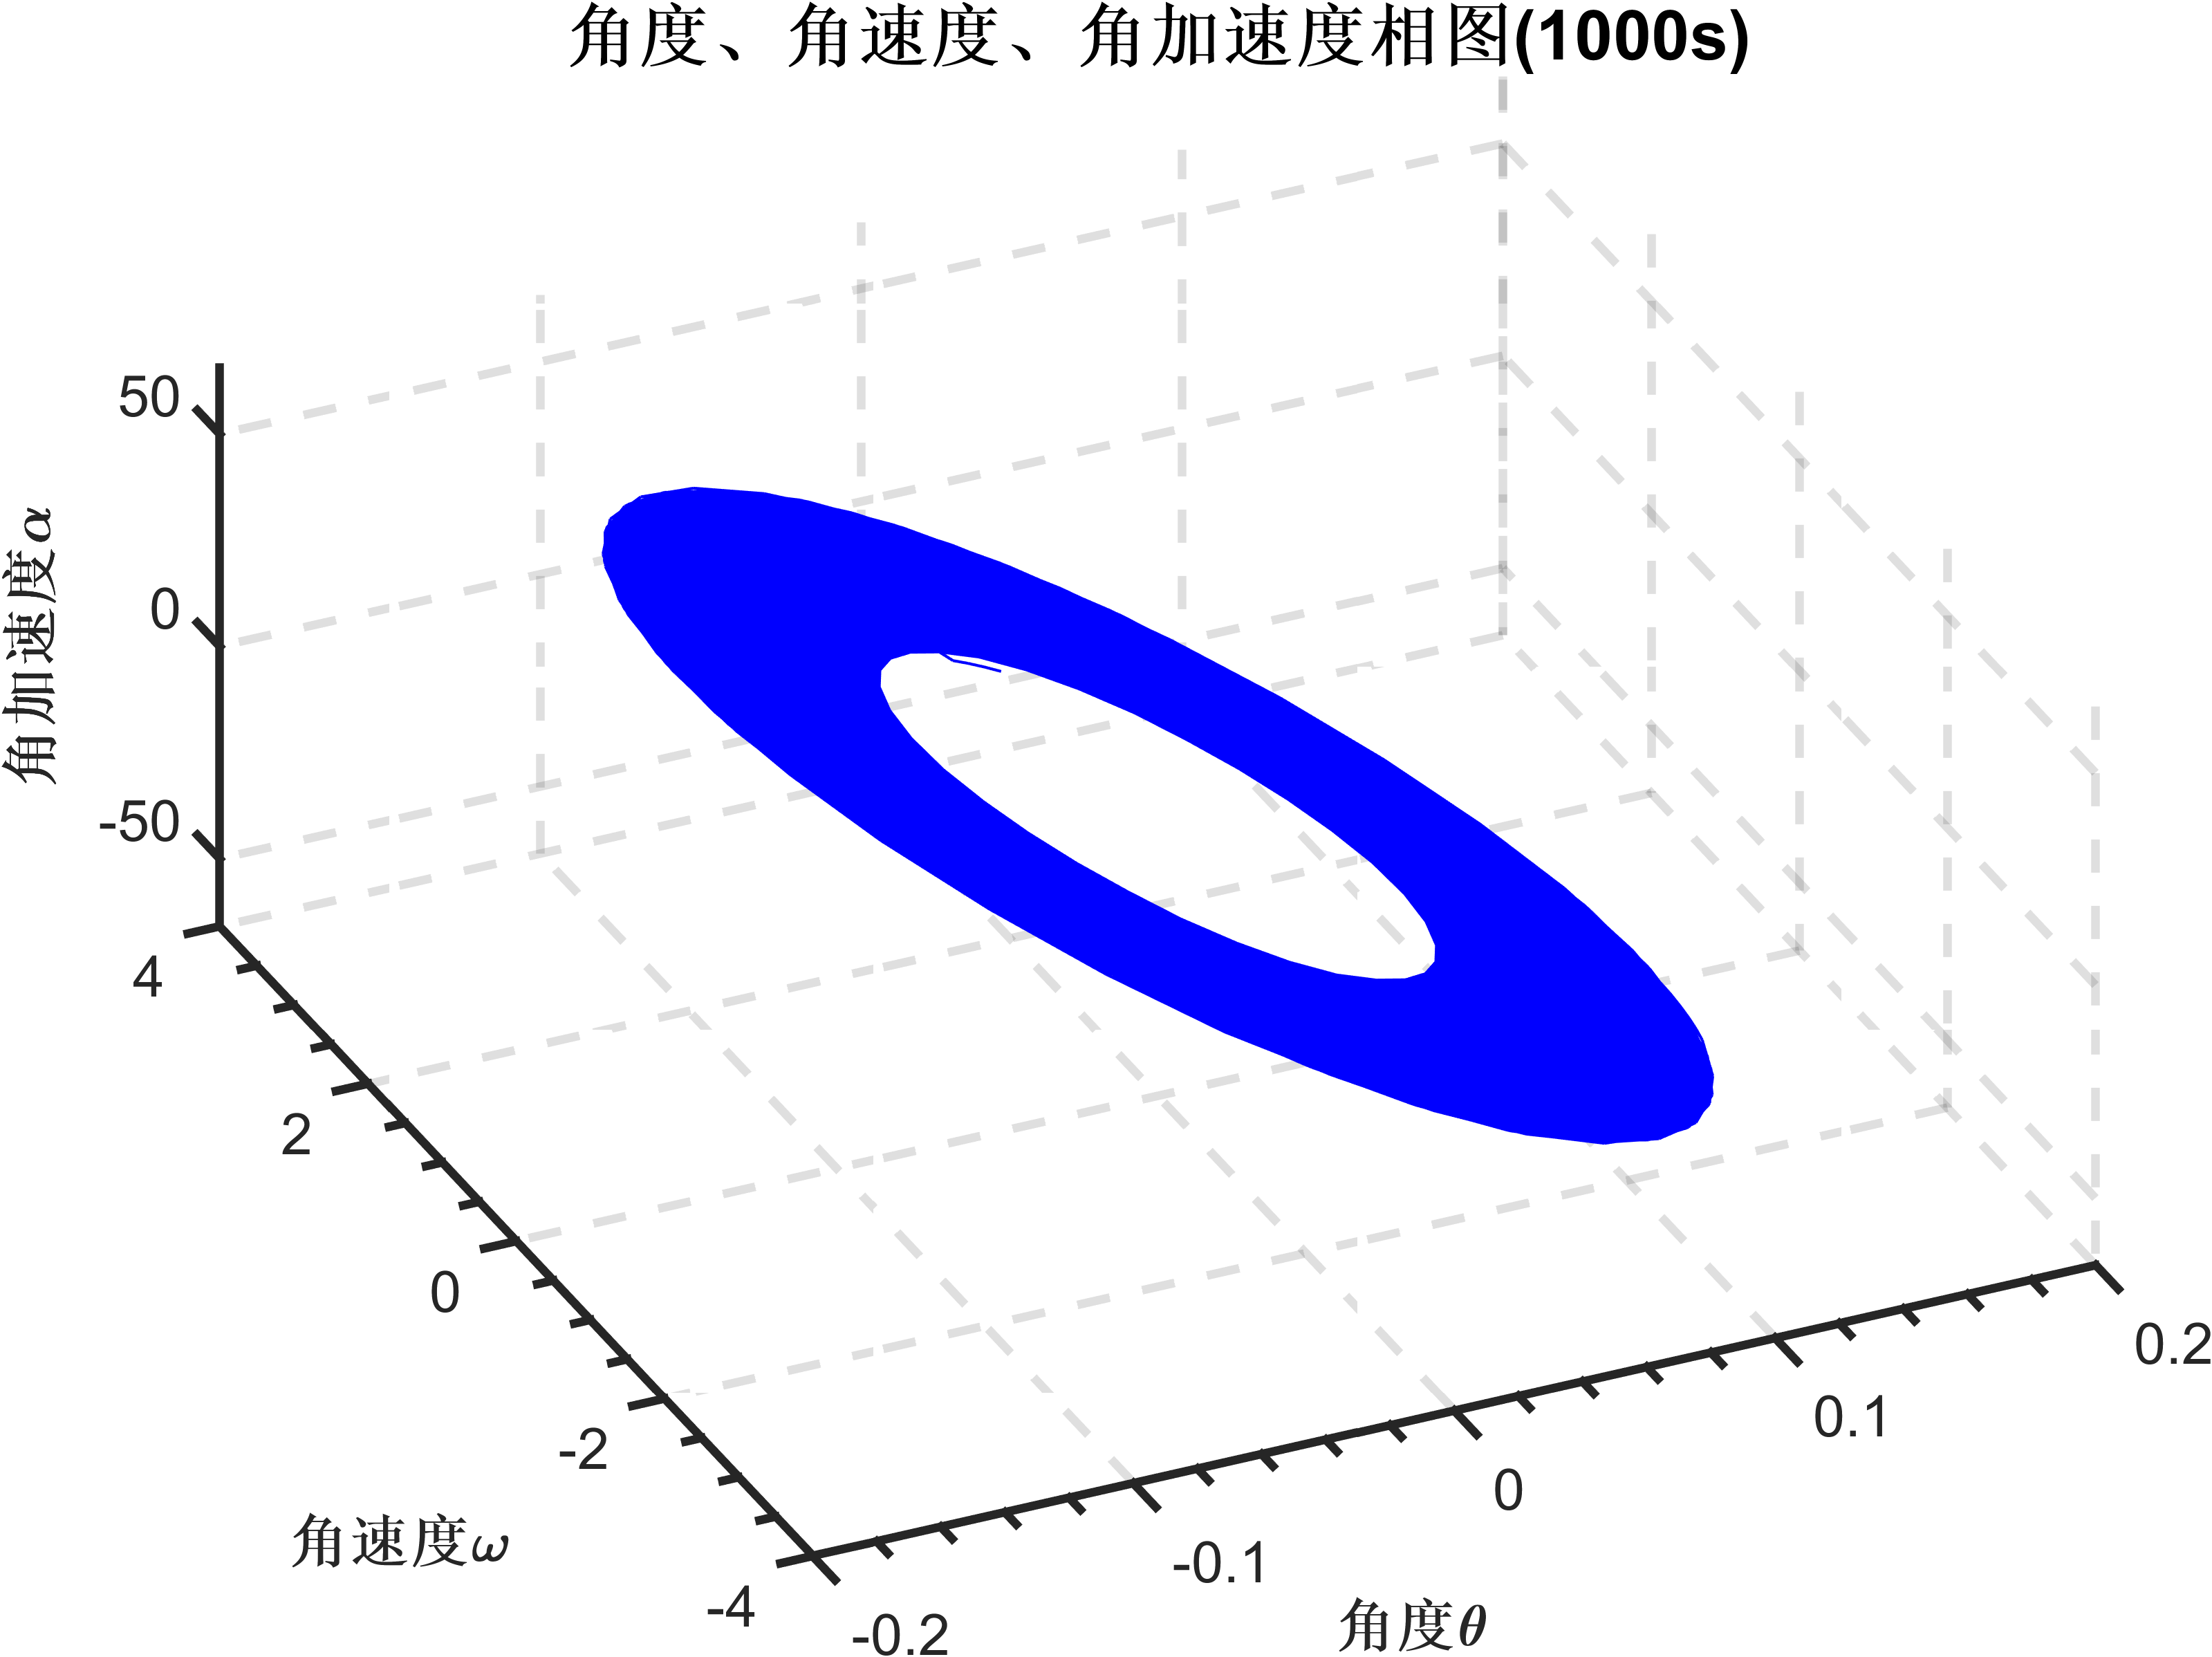
\includegraphics[width=0.6\textwidth]{模型1角度角速度角加速度相图1000s}
	\caption{模型1 1000s内角度、角速度、角加速度的相图}
	\label{模型1角度角速度角加速度相图1000s}
	\end{figure}
	\subsection{模型的近似:近似解析解}
	由问题一的结果可知,当外力$F=50$时,得到的$\theta$值很小。如图\ref{问题2受力示意图theta趋于0}
	 \begin{figure}[H]
		\centering
		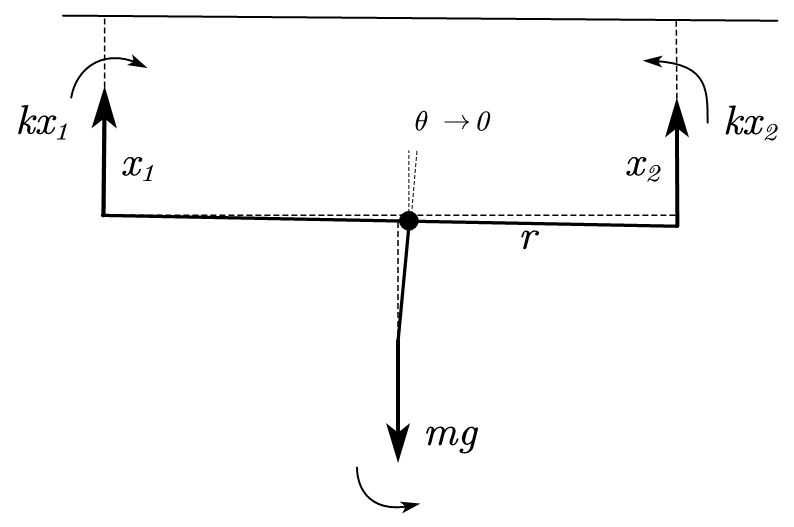
\includegraphics[width=0.6\textwidth]{问题2受力示意图theta趋于0}
		\caption{$\theta$趋于0时受力示意图}
		\label{问题2受力示意图theta趋于0}
	\end{figure}
	
	当$F$较小,即$\theta$较小时,有$$\sin \theta \approx \theta$$,代入初值问题方程(\ref{czq2}),可得近似方程:
	\begin{equation}\label{jsfc}
	\left\{\begin{array}{l}
	\theta^{\prime \prime}=-\frac{8g}{3 \pi r} \theta-\frac{4 k}{m} \theta=-N \theta\\
	\theta(0)=\theta_{0} \quad \theta^{\prime}(0)=0
	\end{array}\right.
	\end{equation}
	解之,得:
	\begin{equation}\label{jg}
	\theta=\theta_{0} \cos \sqrt{N} t
	\end{equation}
	其中$$
	N=\sqrt{\frac{8g}{3\pi r}+\frac{4 k}{m}}$$
	计算运动周期$T$:
	\begin{equation}\label{zqt}
	T=\frac{2 \pi}{\sqrt{N}}=\frac{2 \pi}{\sqrt{\frac{8g}{3\pi r}+\frac{4 k}{m}}}
	\end{equation}
	可以看出,当$\theta$较小时,周期$T$只与$r,m,k$有关,与$l,F$无关。将$k,m,r$的值代入式(\ref{zqt}),求得理论近似运动周期$T=0.3038s$,与数值解法的结果$T\approx 0.30s$十分相近,验证了模型的正确性。
	
	固定$k,m,r$中的一个,作出周期$T$与另外两个变量的关系如图\ref{周期T与kmr的关系},其中固定变量取题中所给的值,即$k=400,m=5,r=0.3$.
				 \begin{figure}[H]
		\centering
		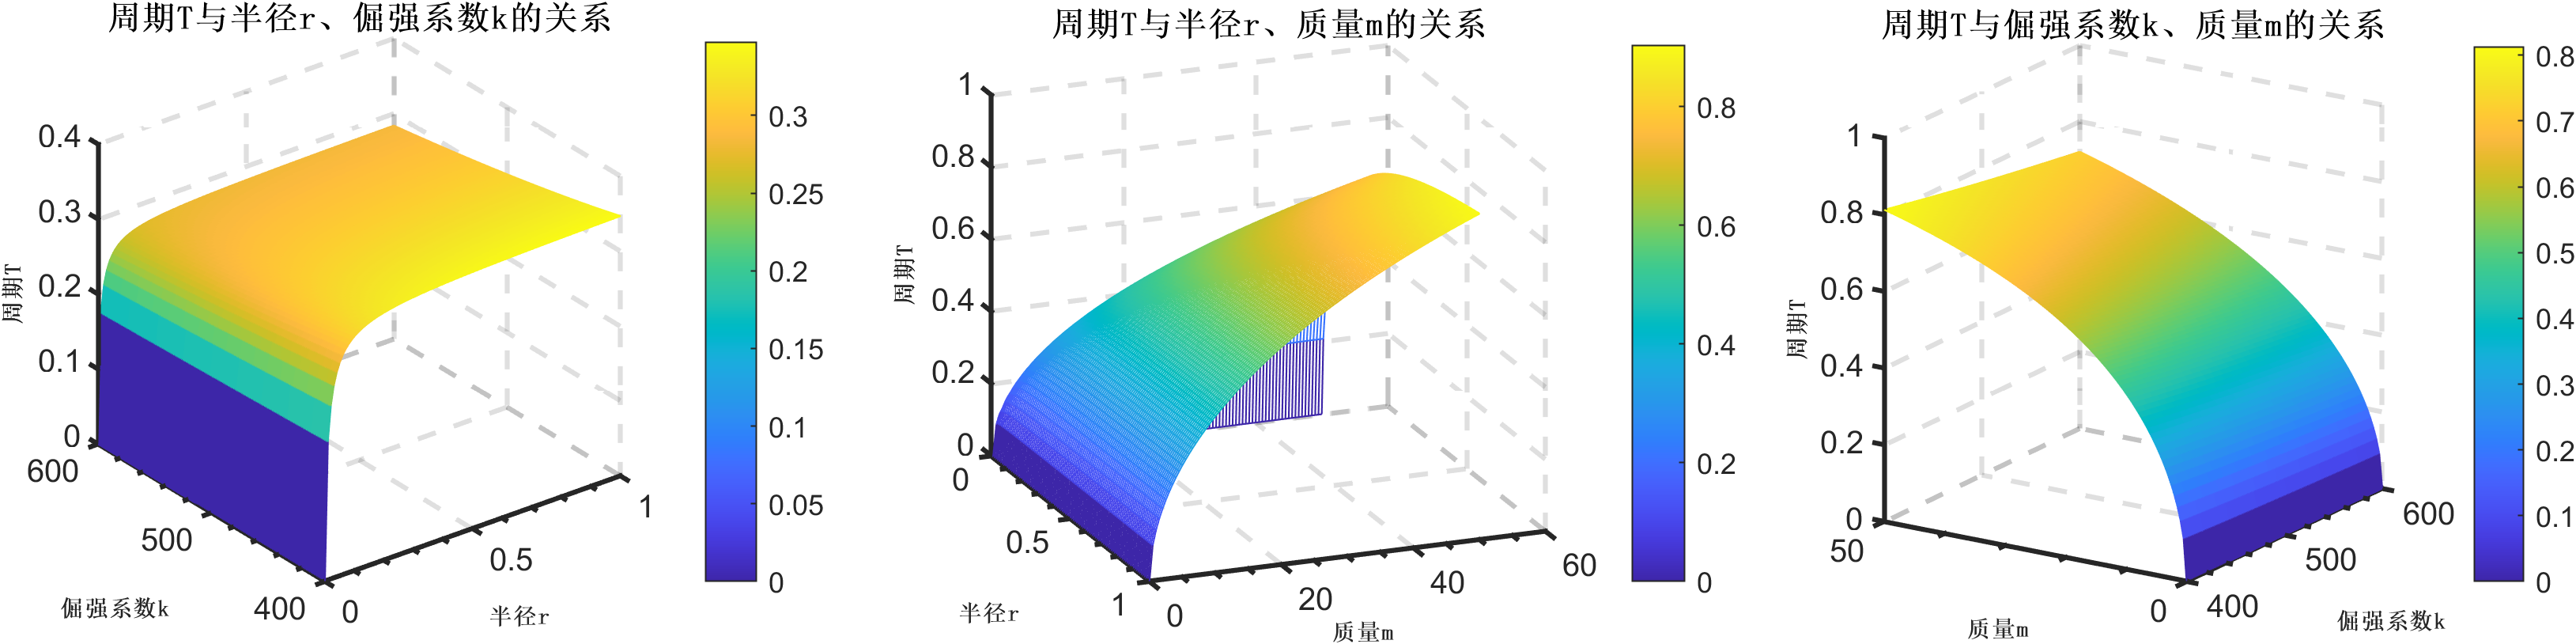
\includegraphics[width=1.0\textwidth]{周期T与kmr的关系}
		\caption{周期$T$与$k,m,r$的关系}
		\label{周期T与kmr的关系}
	\end{figure}
	

	\section{问题三模型}
	\subsection{3-1模型}
	\paragraph{3-1模型的建立}
	同问题一二的模型建立过程相似,设左弹簧与水平线的夹角为$\theta_1$,右弹簧与水平线的夹角为$\theta_2$,将弹簧拉力沿着垂直和水平方向分解,作出受力图:
					 \begin{figure}[H]
		\centering
		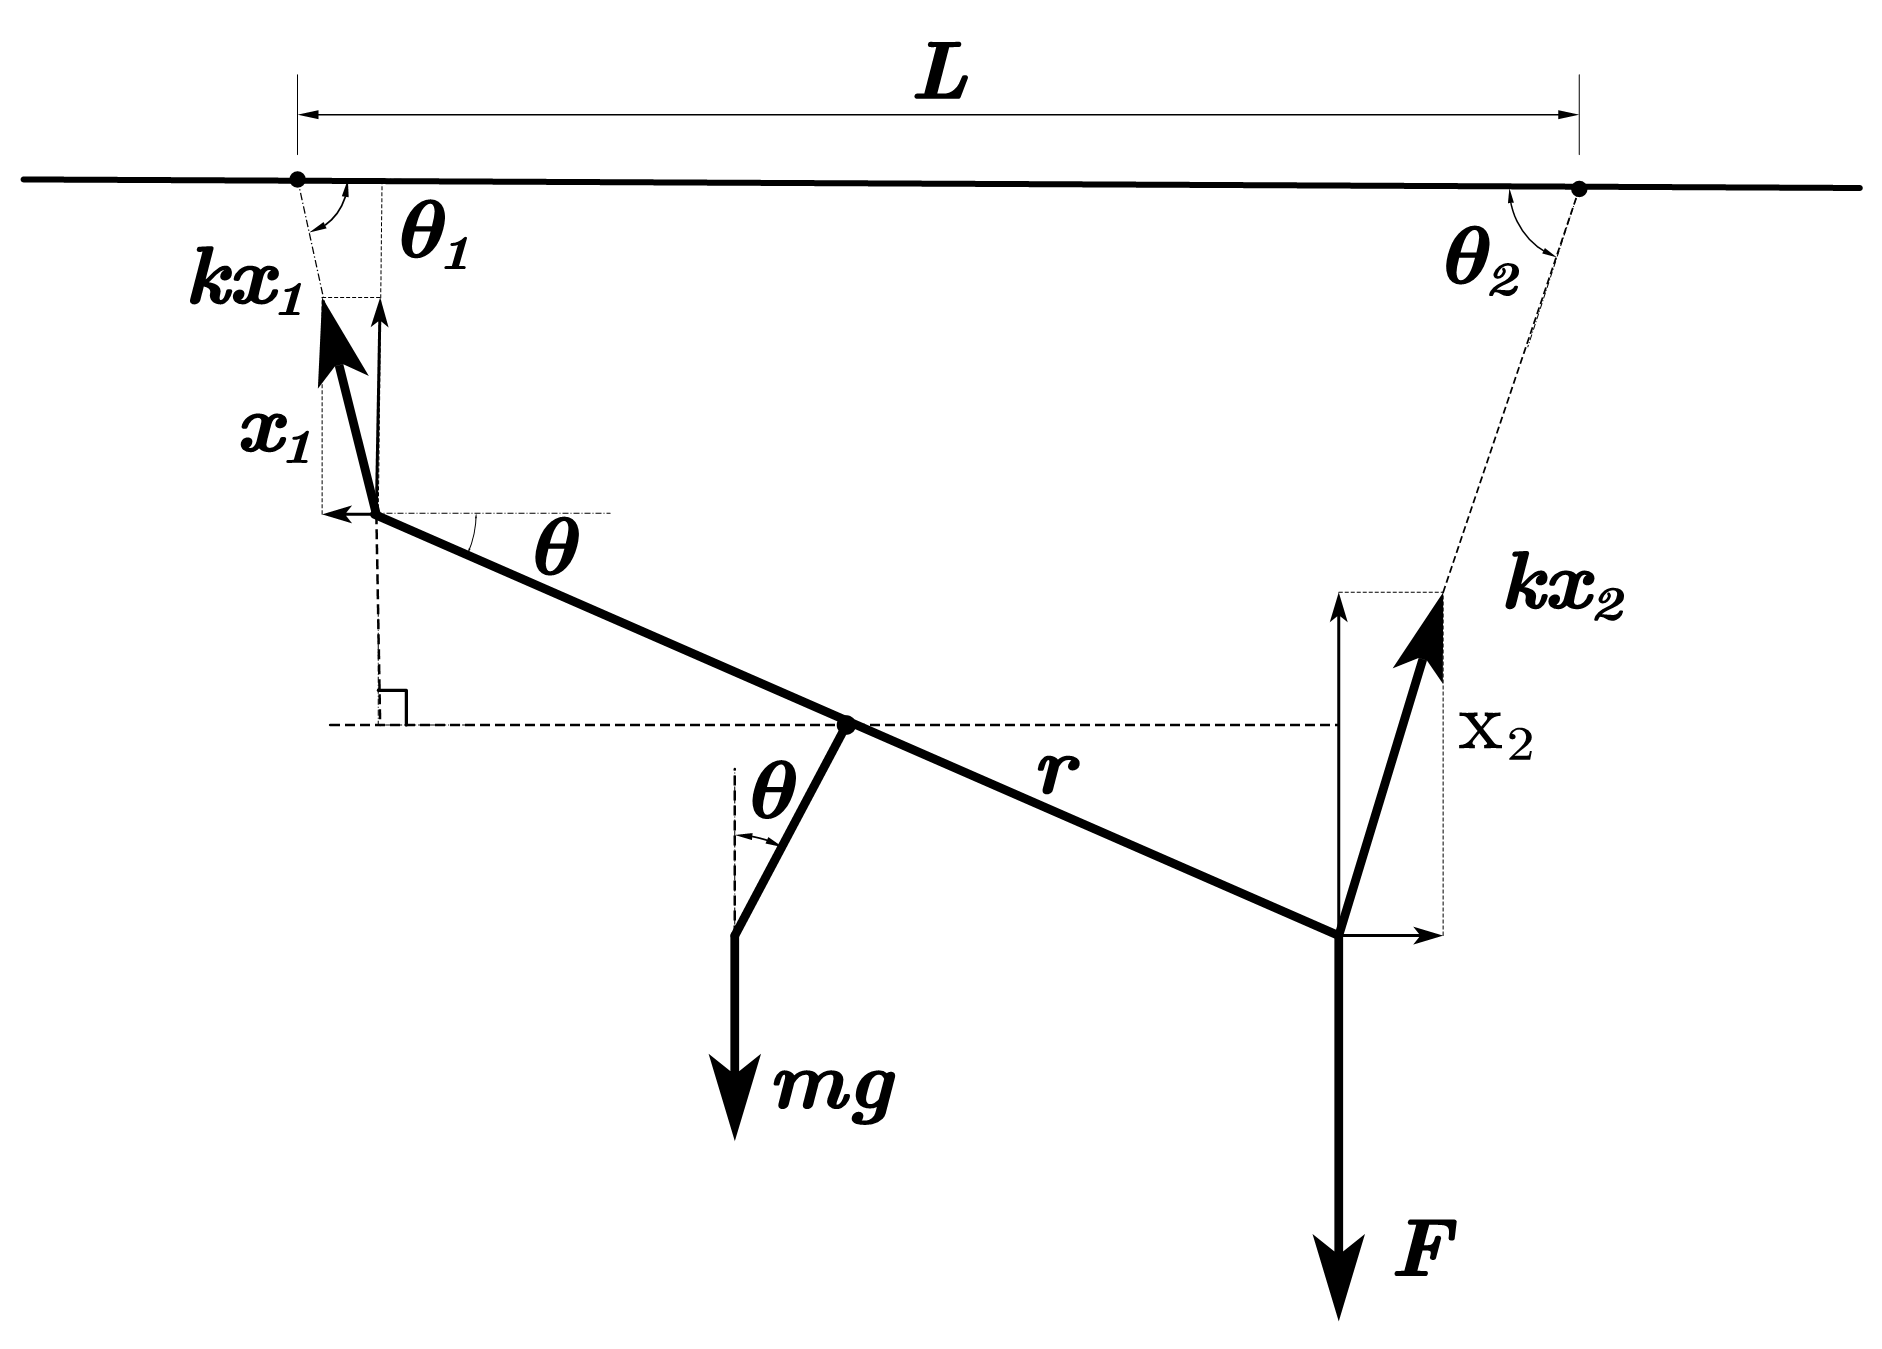
\includegraphics[width=0.55\textwidth]{问题3-1受力示意图}
		\caption{问题3-1受力示意图}
		\label{问题3-1受力示意图}
	\end{figure}
   由几何关系,受力关系,力矩平衡关系写出以下方程组:
	\begin{equation}\label{fczq31}
	\left\{\begin{array}{l}
	\left.\begin{array}{l}
	k x_{2} \cos \theta_{2}=k x_{1} \cos \theta_{1} \\
	k x_{2} \sin \theta_{2}+k x_{1} \sin \theta_{1}=m g+F\\
	\end{array}\right\} \text{受力平衡约束}\\
	\left.\begin{array}{l}
	k x_{2} \cos \theta_{2} r \sin \theta+k x_{1} \cos \theta_{1}r\sin\theta + k x_{2} \sin \theta_{2} r \cos \theta+m g \frac{4 r}{3 \pi} \sin \theta \\
	=F r \cos \theta+k x_{1} \sin \theta_{1} r \cos \theta
	\end{array}\right\} \text{力矩平衡约束}\\
	\left.\begin{array}{l}
	\left(l+x_{1}\right) \cos \theta_{1}+\left(l+x_{2}\right) \cos \theta_{2}+2 r \cos \theta =L\\
	\left(l+x_{1}\right) \sin \theta_{1}+2 r \sin \theta=\left(l+x_{2}\right) \sin \theta_{2}
	\end{array}\right\} \text{几何约束}\\
	\end{array}\right.
	\end{equation}
\paragraph{3-1模型的求解}
使用数值法求解方程组(\ref{fczq31}),使用fsolve函数,设置$\theta,\theta^{\prime},x_1,x_2,\theta_1,\theta_2$的初值分别为$0,0,0,0,\pi/2,\pi/2$,迭代求解,解得$\theta=0.1562,x_1=0.0524,x_2=0.1456,\theta_1 =1.5615,\theta_2 =1.5675$.
	\subsection{3-2模型}
	\paragraph{3-2模型的建立}
	作出撤去外力F之后的受力情况,如图
 	\begin{figure}[H]
		\centering
		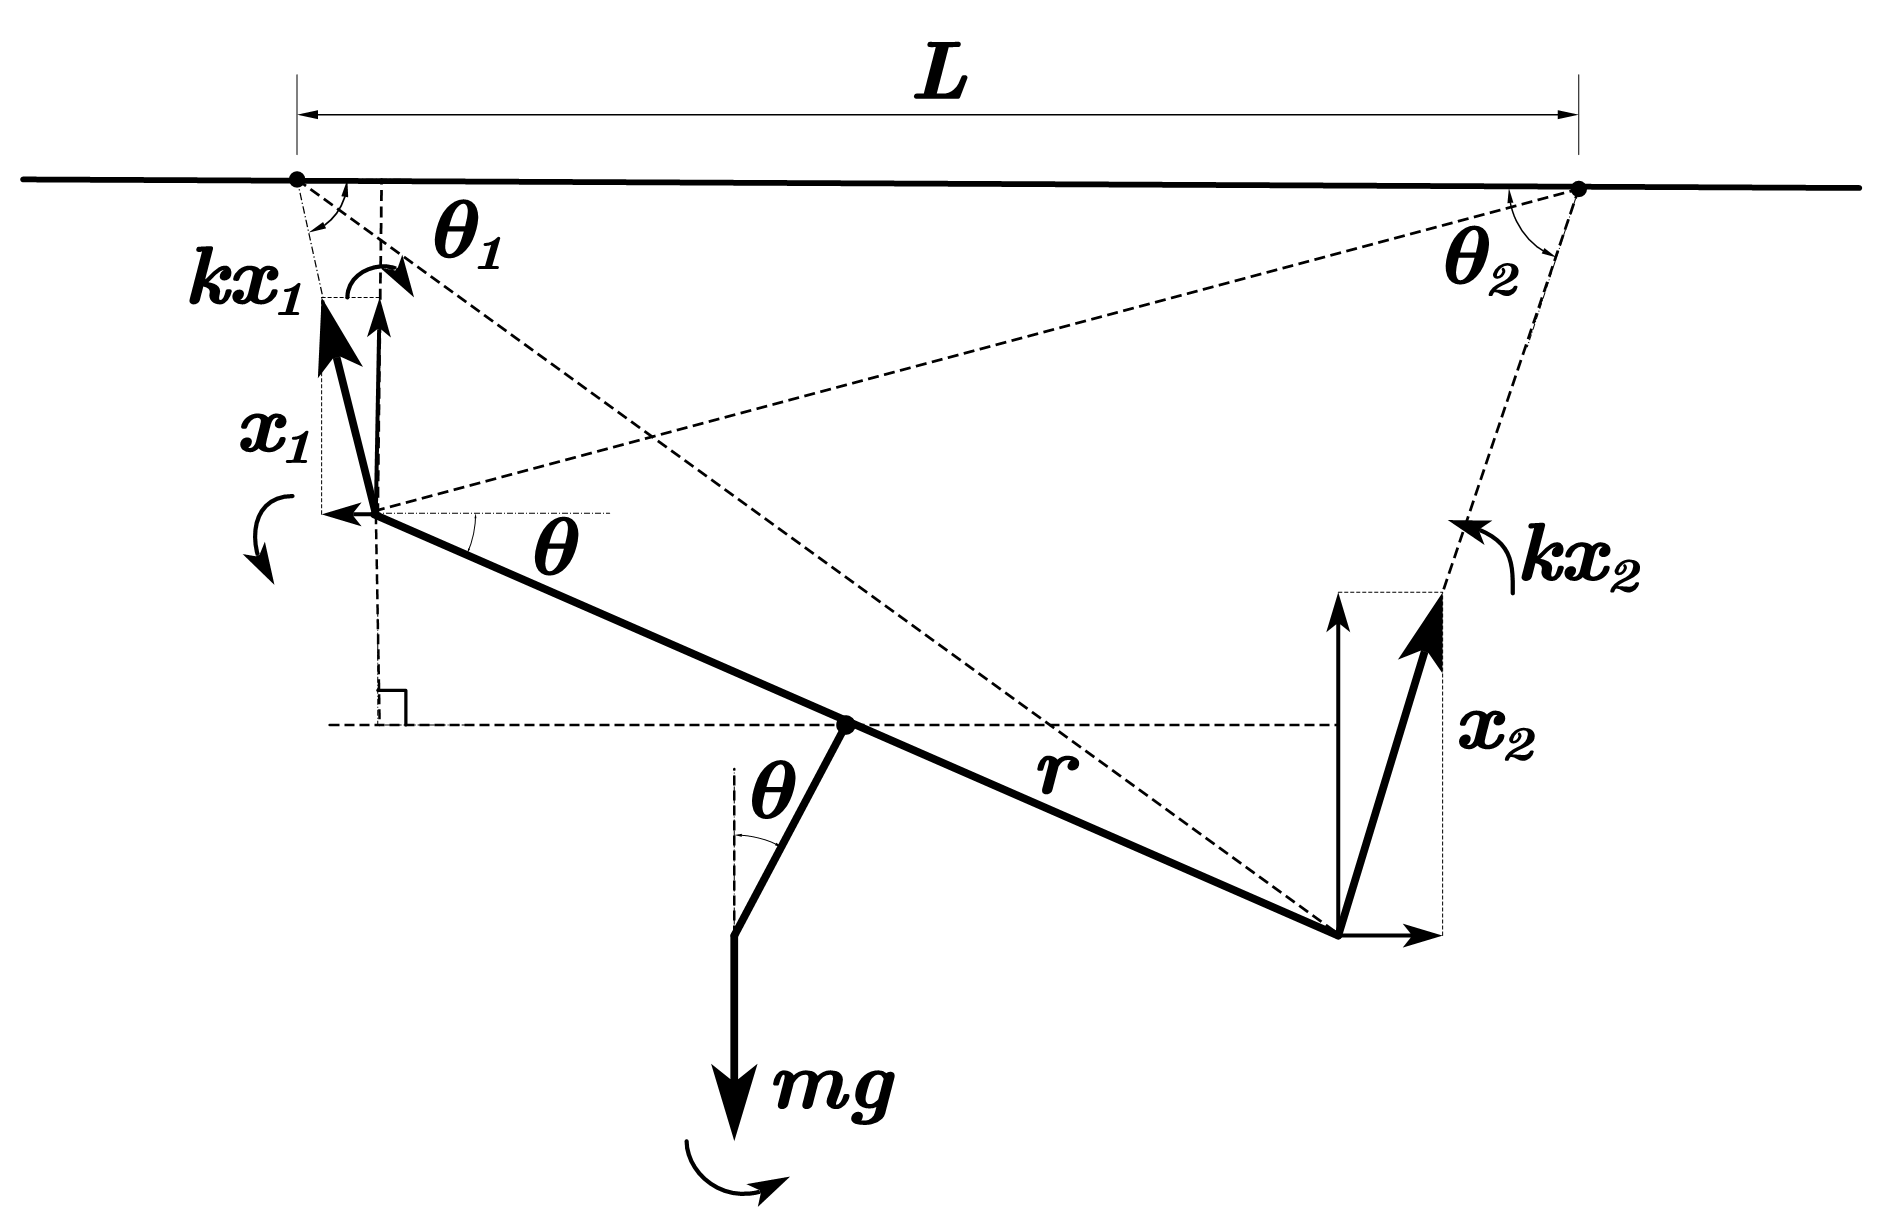
\includegraphics[width=0.55\textwidth]{问题3-2受力示意图}
		\caption{问题3-2受力示意图}
		\label{问题3-2受力示意图}
	\end{figure}
	由转动定理,可得:
	\begin{equation}\label{zddlq3}
	\begin{aligned}
	&k x_{2} \cos \theta_{2} r \sin \theta+k x_{1} \cos \theta_{1} r \sin \theta+k x_{2} \sin \theta_{2} r \cos \theta+m g \frac{4 r}{3 \pi} \sin \theta-k x_{1} \sin \theta_{1} r \cos \theta \\
	&=-\frac{m r^{2}}{2} \theta^{\prime \prime}
	\end{aligned}
	\end{equation}
	由余弦定理,增加两条几何约束:
	\begin{equation}\label{xzjhys}
	\left\{\begin{array}{l}
	L^{2}+\left(l+x_{2}\right)^{2}-2\left(l+x_{2}\right) L \cos \theta_{2}=4 r^{2}+\left(l+x_{1}\right)^{2}+4\left(l+x_{1}\right) r \cos \left(\theta_{1}-\theta\right) \\
	L^{2}+\left(l+x_{1}\right)^{2}-2\left(l+x_{1}\right) L \cos \theta_{1}=4 r^{2}+\left(l+x_{2}\right)^{2}+4\left(l+x_{2}\right) r \cos \left(\theta_{2}+\theta\right) 
	\end{array}\right.
	\end{equation}
	式(\ref{xzjhys}) 与式(\ref{fczq31}) 中的两条几何约束共同构成一组完备的约束,以求解微分方程(\ref{zddlq3}) .

	同样,令$\theta^{\prime}=\omega$,$\omega$为角速度,将二阶导数转化为两个一阶导数,得到如下初值问题:
	\begin{equation}\label{wfdsfc}
	\left\{\begin{array}{l}
	
	\theta^{\prime}=\omega \\
	\omega^{\prime}=f\left(x_{1}, x_{2}, \theta_{1}, \theta_{2}, \theta\right)\\
	\theta(0)=\theta_0,\omega(0)=0\\
	x_1(0)={x_1}_0, x_2(0)={x_2}_0\\ 
	\theta_1(0)={\theta_1}_0,\theta_2(0)={\theta_2}_0
	
	\end{array}\right.
	\end{equation}
	分别将式(\ref{fczq31}) 中的几何约束、式(\ref{zddlq3})、式(\ref{xzjhys})移项获得函数$f,g,\varepsilon,\psi,\eta$:
	
	\begin{equation}\label{wfdsfc2}
	\left\{\begin{array}{l}
	0=g\left(x_{1}, x_{2}, \theta_{1}, \theta_{2}, \theta\right) \\
	0=\varepsilon\left(x_{1}, x_{2}, \theta_{1}, \theta_{2}, \theta\right) \\
	0=\psi\left(x_{1}, x_{2}, \theta_{1}, \theta_{2}, \theta\right) \\
	0=\eta\left(x_{1}, x_{2}, \theta_{1}, \theta_{1}, \theta\right)
	\end{array}\right.
	\end{equation}
	
		\paragraph{3-2模型的求解}
		\subsubsection{求解方法1:ode15s}
	式(\ref{wfdsfc}) 和式(\ref{wfdsfc2})是微分代数方程,将式(\ref{wfdsfc}) 和式(\ref{wfdsfc2})联立,化为矩阵形式:
	\begin{equation}\label{jzxs}
	M\left[\begin{array}{c}
	\theta^{\prime} \\
	\omega^{\prime} \\
	x_{1}^{\prime} \\
	x_{2}^{\prime} \\
	\theta_{1}^{\prime} \\
	\theta_{2}^{\prime}
	\end{array}\right]=\left[\begin{array}{ccccc}
	1 & 0 & \cdots & \cdots & 0 \\
	0 & 1 & \cdots & \cdots & \vdots \\
	\vdots & \vdots & \ddots & \vdots & \vdots \\
	\vdots & \vdots & \cdots & 0 & \vdots \\
	0 & \cdots & \cdots & \cdots & 0
	\end{array}\right]\left[\begin{array}{c}
	\theta^{\prime} \\
	\omega^{\prime} \\
	x_{1}^{\prime} \\
	x_{2}^{\prime} \\
	\theta_{1}^{\prime} \\
	\theta_{2}^{\prime}
	\end{array}\right]=\left[\begin{array}{c}
	\omega \\
	f \\
	g \\
	\varepsilon \\
	\phi \\
	\eta
	\end{array}\right]
	\end{equation}
	其中M为奇异质量矩阵,利用ode15s函数求解,

	\subsubsection{求解方法2:迭代法+ode45}
	给定$\theta$值,由式(\ref{wfdsfc2})方程组可确定$x_{1}, x_{2}, \theta_{1}, \theta_{2}$的值,函数$\Psi$由式(\ref{wfdsfc2})确定。
	\begin{equation}\label{key}
	\theta= \Psi\left( x_1,x_2,\theta_1,\theta_2\right)
	\end{equation}
	
	因此,先求解代数方程,然后代入微分项更新导数。步骤如下:
	
	给定新的$\theta$的值,以以前的$x_1,x_2,\theta_1,\theta_2$作为初值,代入$\Psi\left( x_1,x_2,\theta_1,\theta_2\right)$,求解新的$x_1,x_2,\theta_1,\theta_2$,进行迭代,并使用ode45函数求解下式:
	\begin{equation}\label{xs}
	\left\{\begin{array}{l}
	\begin{aligned}
	&\theta^{\prime}=\omega \\
	&\omega^{\prime}=f\left(x_{1}, x_{2}, \theta_{1}, \theta_{2}, \theta\right) \\
	&\theta(0)=\theta_0,\omega(0)=0
	\end{aligned}
	\end{array}\right.
	\end{equation}
	
	\subsubsection{3-2模型求解结果}
	由上述求解方法,求微分代数方程的数值解,作出角度$\theta$与角速度$\theta^{\prime}$的变化关系:
 	\begin{figure}[H]
		\centering
		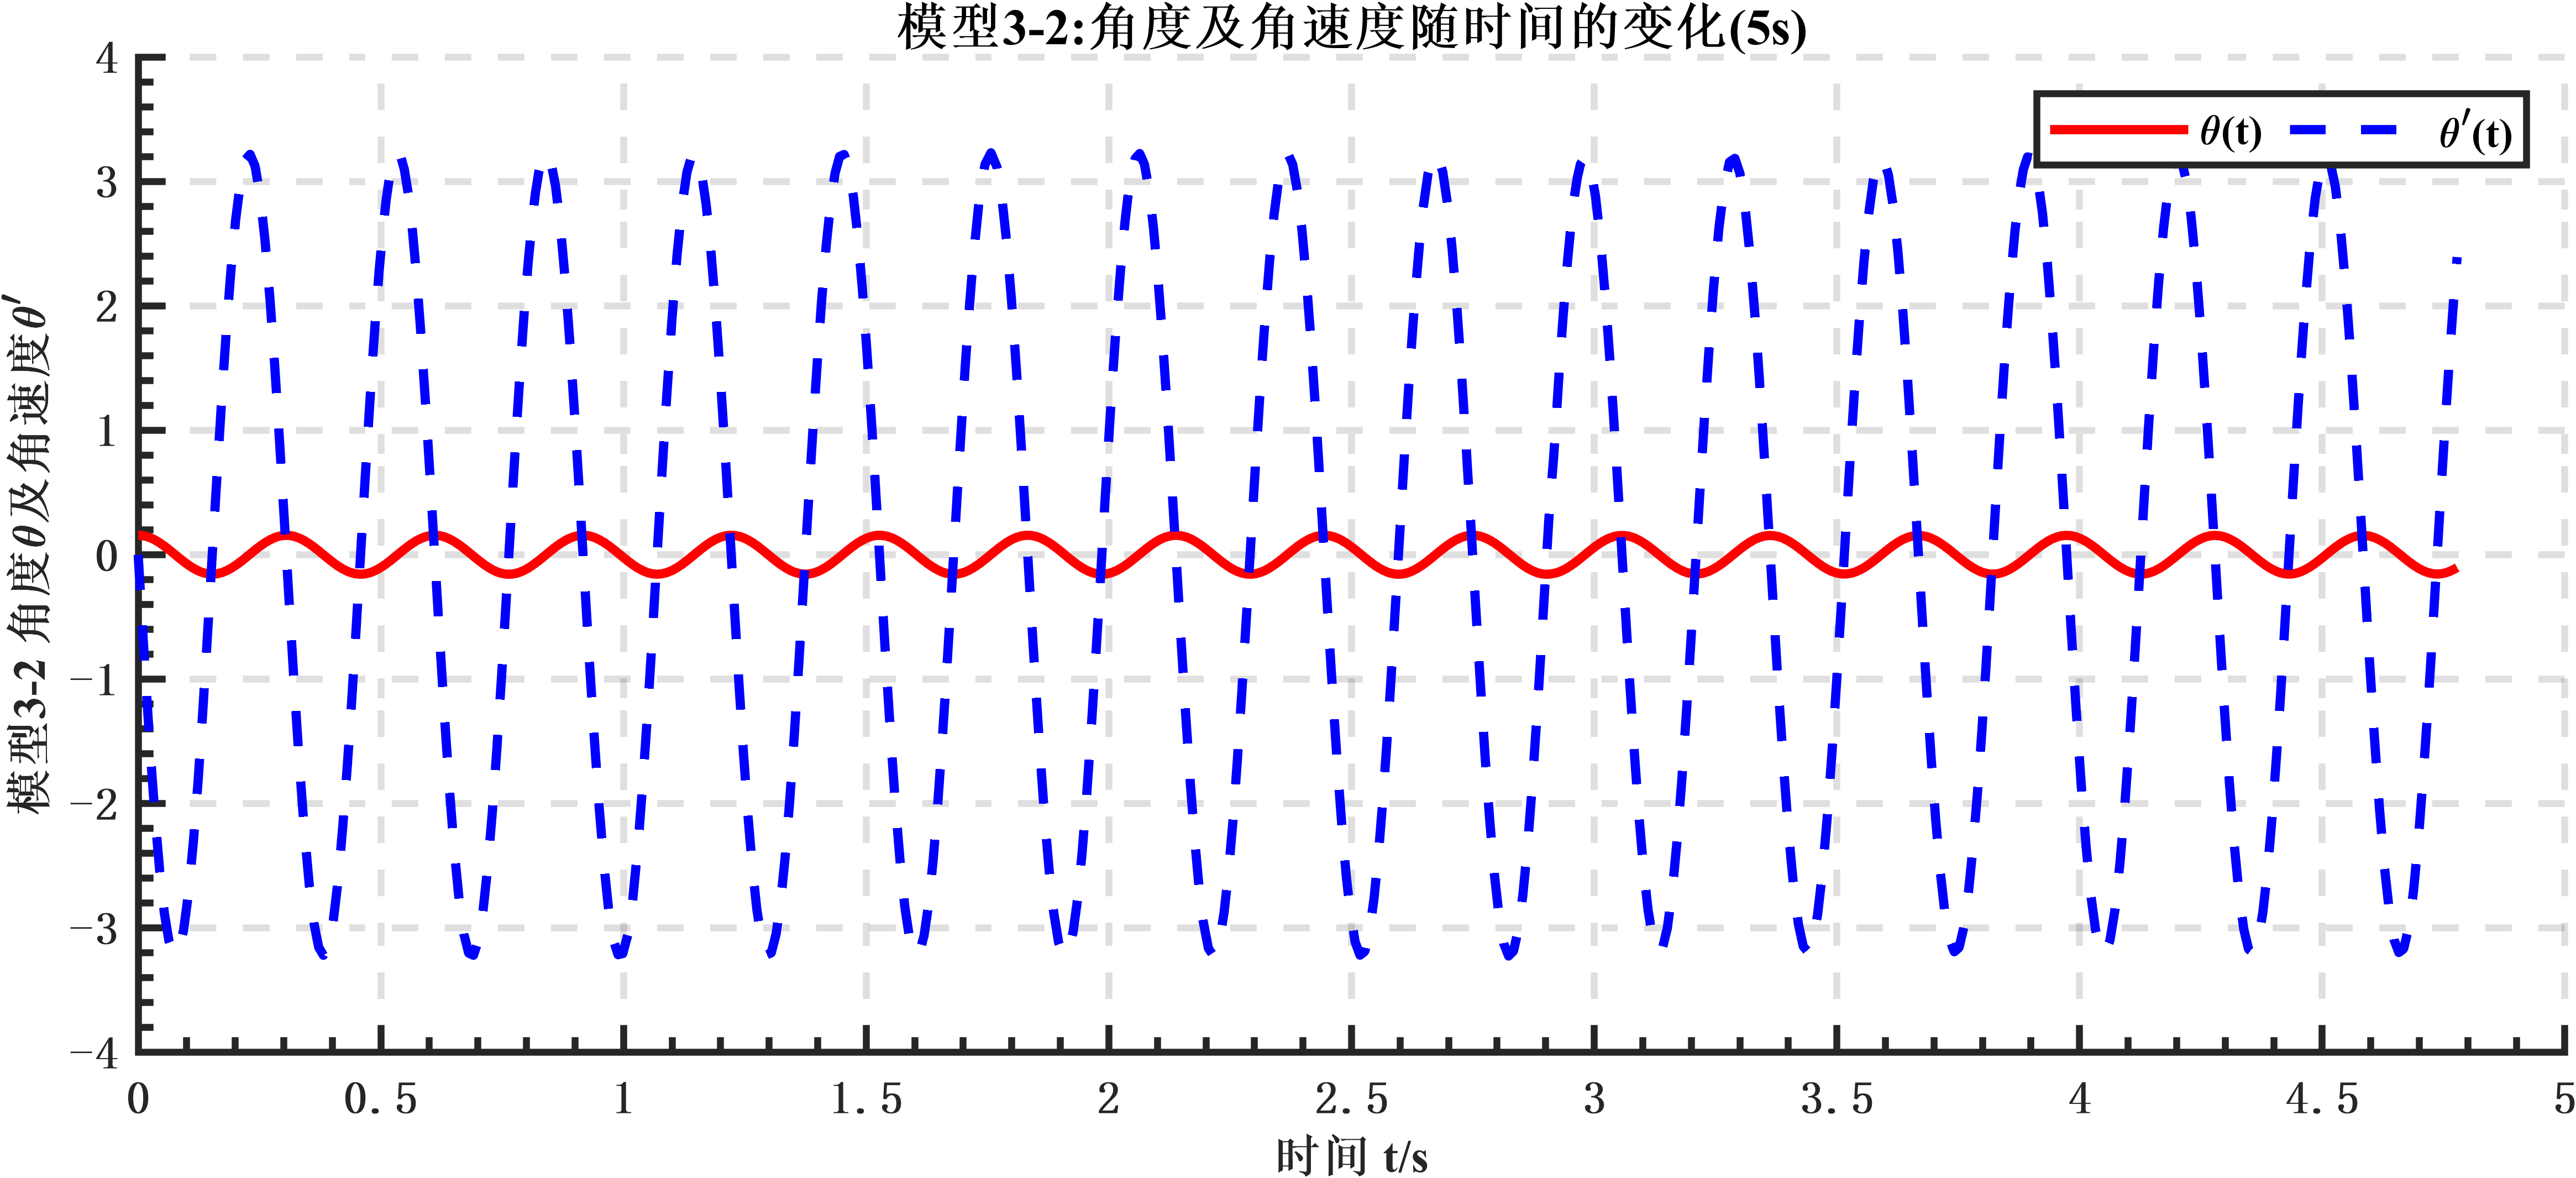
\includegraphics[width=0.85\textwidth]{模型3-2角度及角速度随时间的变化5s}
		\caption{模型3-2:角度及角速度随时间的变化(5s)}
		\label{模型3-2角度及角速度随时间的变化5s}
	\end{figure}

 	\begin{figure}[H]
	\centering
	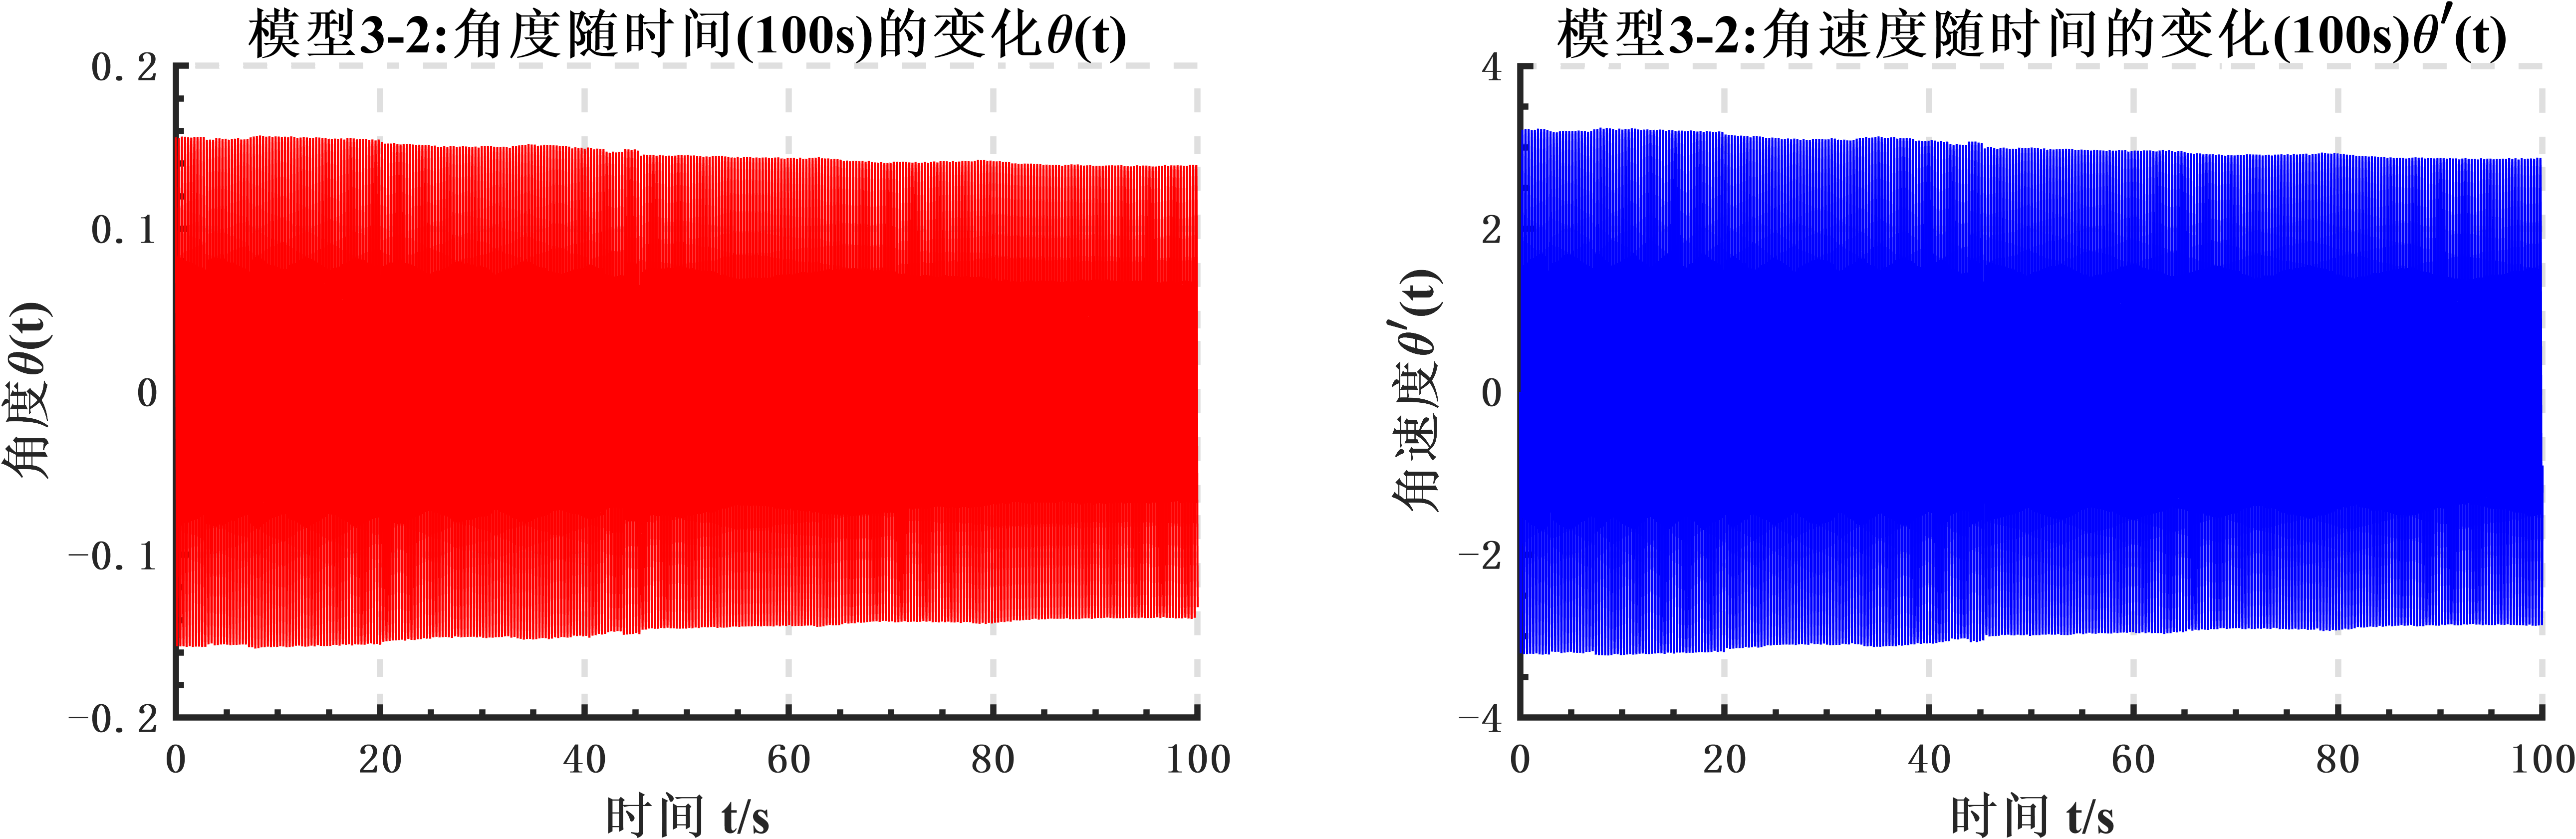
\includegraphics[width=0.9\textwidth]{模型3-2角度及角速度随时间的变化100s}
	\caption{模型3-2:角度及角速度随时间的变化(100s)}
	\label{模型3-2角度及角速度随时间的变化100s}	
	\end{figure}
	\subsubsection{3-2模型的近似解析解}
	当$F$较小,即$\theta$较小时,有$$\sin \theta \approx \theta,x_1 \approx x_2 ,\theta_1 \approx \theta_2 $$,
	 	\begin{figure}[H]
		\centering
		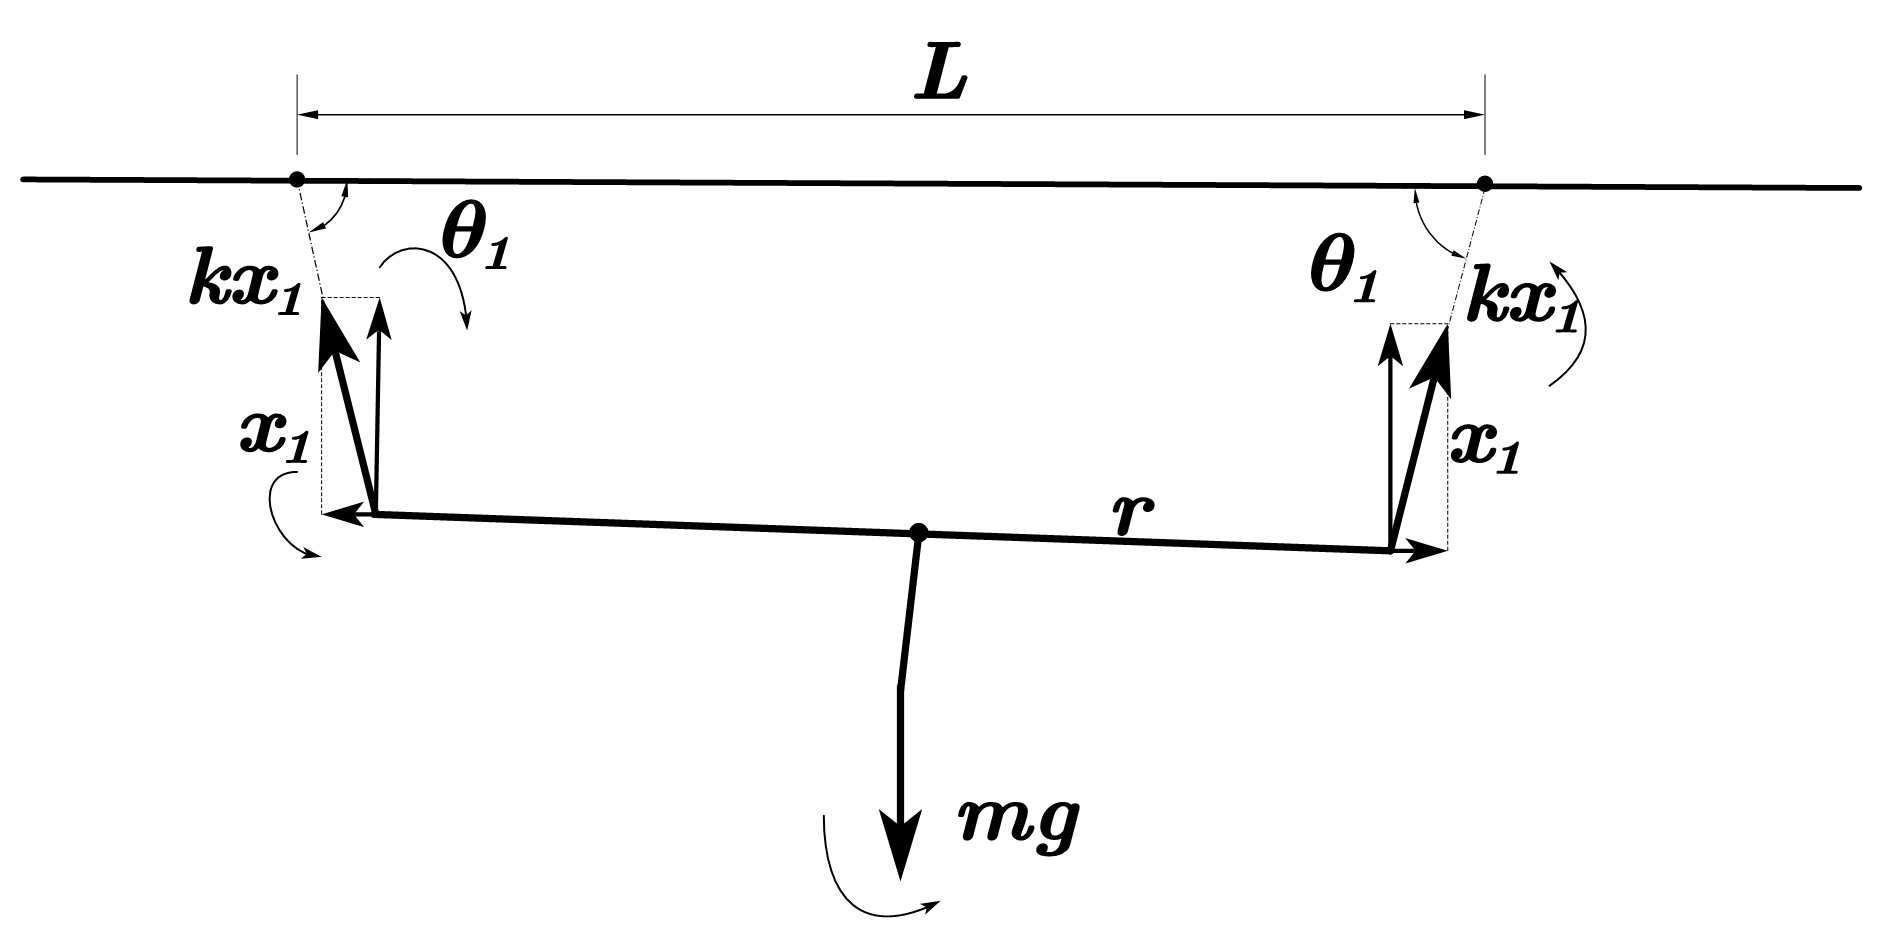
\includegraphics[width=0.6\textwidth]{问题3-2受力示意图theta趋于0}
		\caption{问题3-2:$\theta$趋于0时受力示意图}
		\label{问题3-2受力示意图theta趋于0}
	\end{figure}
	
	代入初值问题方程(\ref{wfdsfc})(\ref{wfdsfc2}),可得近似方程:
	\begin{equation}\label{jsfcq3}
	\left\{\begin{array}{l}
	2 k x_{1} \cos \theta_{1} \theta+m g \frac{4}{3 \pi} \theta=-\frac{m r}{2} \theta^{\prime \prime} \\
	2\left(l+x_{1}\right) \cos \theta_{1}+2 r=L \\
	2 k x_{1} \sin \theta_{1}=m g 
	\end{array}\right.
	\end{equation}
	化简得:
	\begin{equation}\label{tc}
	\begin{aligned}
	\Rightarrow \theta^{\prime \prime} &=-\left[m g \frac{4}{3 \pi}+\Omega(r, m, k, l, L)\right] \theta \\
	&=-N \theta
	\end{aligned}
	\end{equation}
	其中函数$\Omega$是关于$(r, m, k, l, L)$的方程,由式(\ref{jsfcq3})可确定。解式(\ref{tc})得:
	\begin{equation}\label{jd}
	\begin{aligned}
	&\Rightarrow \theta^{\prime}=\theta_{0} \cos \sqrt{N} t \\
	&T=\frac{2 \pi}{\sqrt{N}}=\frac{2 \pi}{\sqrt{\frac{8g}{3 \pi r}+\Omega(r, m, k, l, L)}}
	\end{aligned}
	\end{equation}
	由于题中$2 r = 0.6,L=0.6$,即$2r=L$,代入式(\ref{jsfcq3}) ,可得$\theta_1 \approx \pi/2$,于是式(\ref{zddlq3}) 、式(\ref{wfdsfc2}) 化简得:
		\begin{equation}\label{jsfc2}
	\left\{\begin{array}{l}
	\theta^{\prime \prime}=-\frac{8g}{3 \pi r} \theta-\frac{4 k}{m} \theta=-N \theta\\
	\theta(0)=\theta_{0} \quad \theta^{\prime}(0)=0
	\end{array}\right.
	\end{equation}
	上式与式(\ref{jsfc}) 相同,这就是两个角度随时间演化模型的图像(图\ref{模型3-2角度及角速度随时间的变化5s}和图\ref{模型1角度及角速度随时间的变化})相似的原因。
	
	
	
	
	
	\section{模型的推广}
	前文提出的角度时间演化模型基于半圆形薄片绕过圆心且垂直于薄片的直线作定轴转动的假设,只适用于初始角度较小的短期变化情形。模型推导出的长期变化情况与实际不符。
	
	前文已经说到,出现这种情况的原因在于,实际上半圆形薄片作的并不是定轴运动,系统不仅仅有转动,还有竖直方向的运动,参考点圆心的位置随着时间变化,而模型是基于定轴运动建立的,这就导致了能量不守恒的假象。现考虑实际情况:
	
	同时考虑转动和竖直方向运动,作出问题二及问题3-2示意图如图\ref{问题2实际情况},\ref{问题3-2实际情况1},\ref{问题3-2实际情况2},其中问题3-2分为普通情况($L \neq 2r$)和题给条件下$L=2r$的情况。

\begin{figure}[H]
	\centering
	\begin{minipage}[c]{0.48\textwidth}
		\centering
		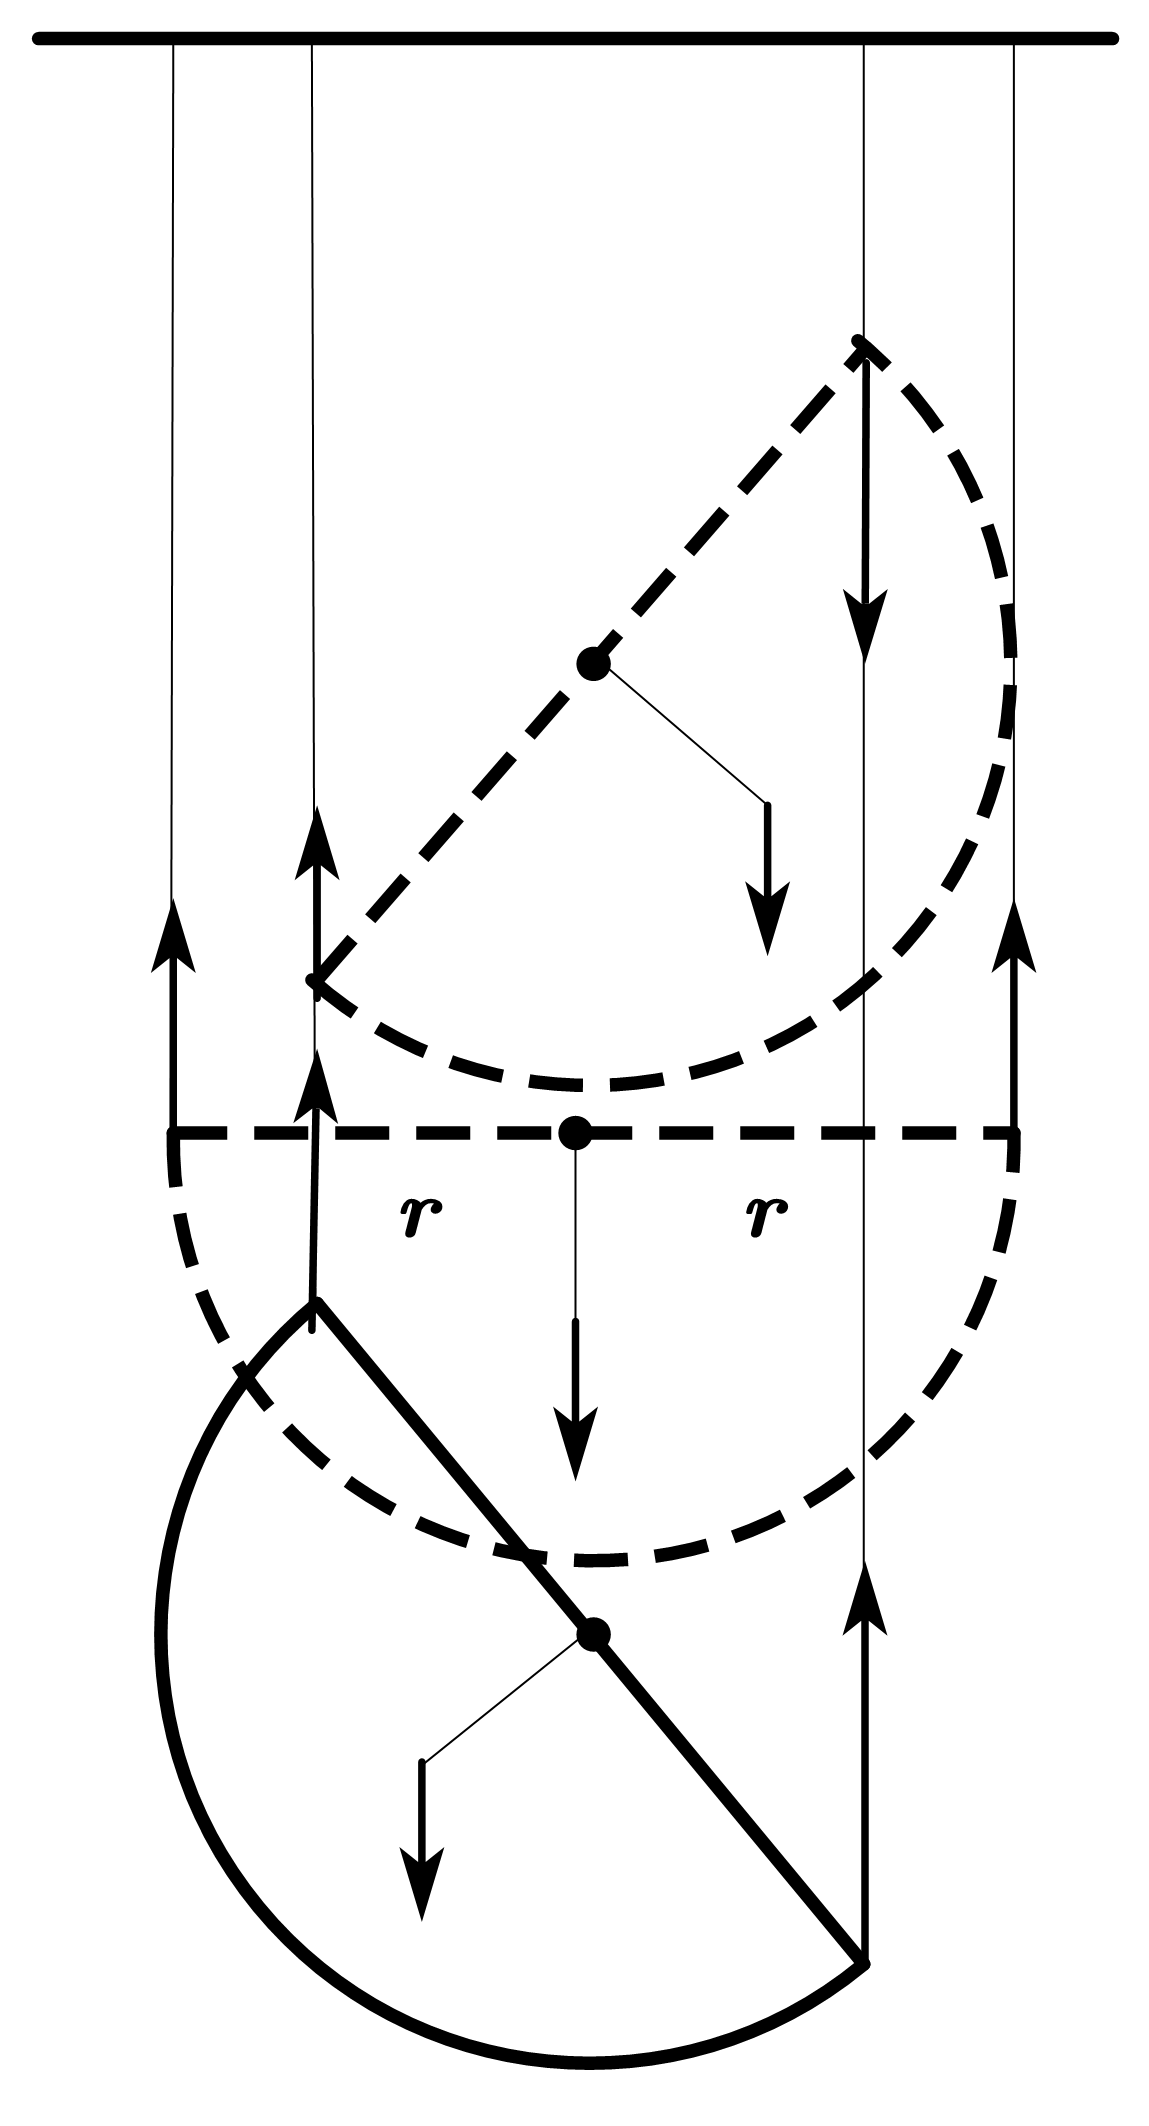
\includegraphics[height=0.3\textheight]{问题2实际情况}
		\caption{问题2\quad$\theta$角较大时实际变化情况示意图}
		\label{问题2实际情况}
	\end{minipage}%
	\hfill
	\begin{minipage}[c]{0.48\textwidth}
		\centering
		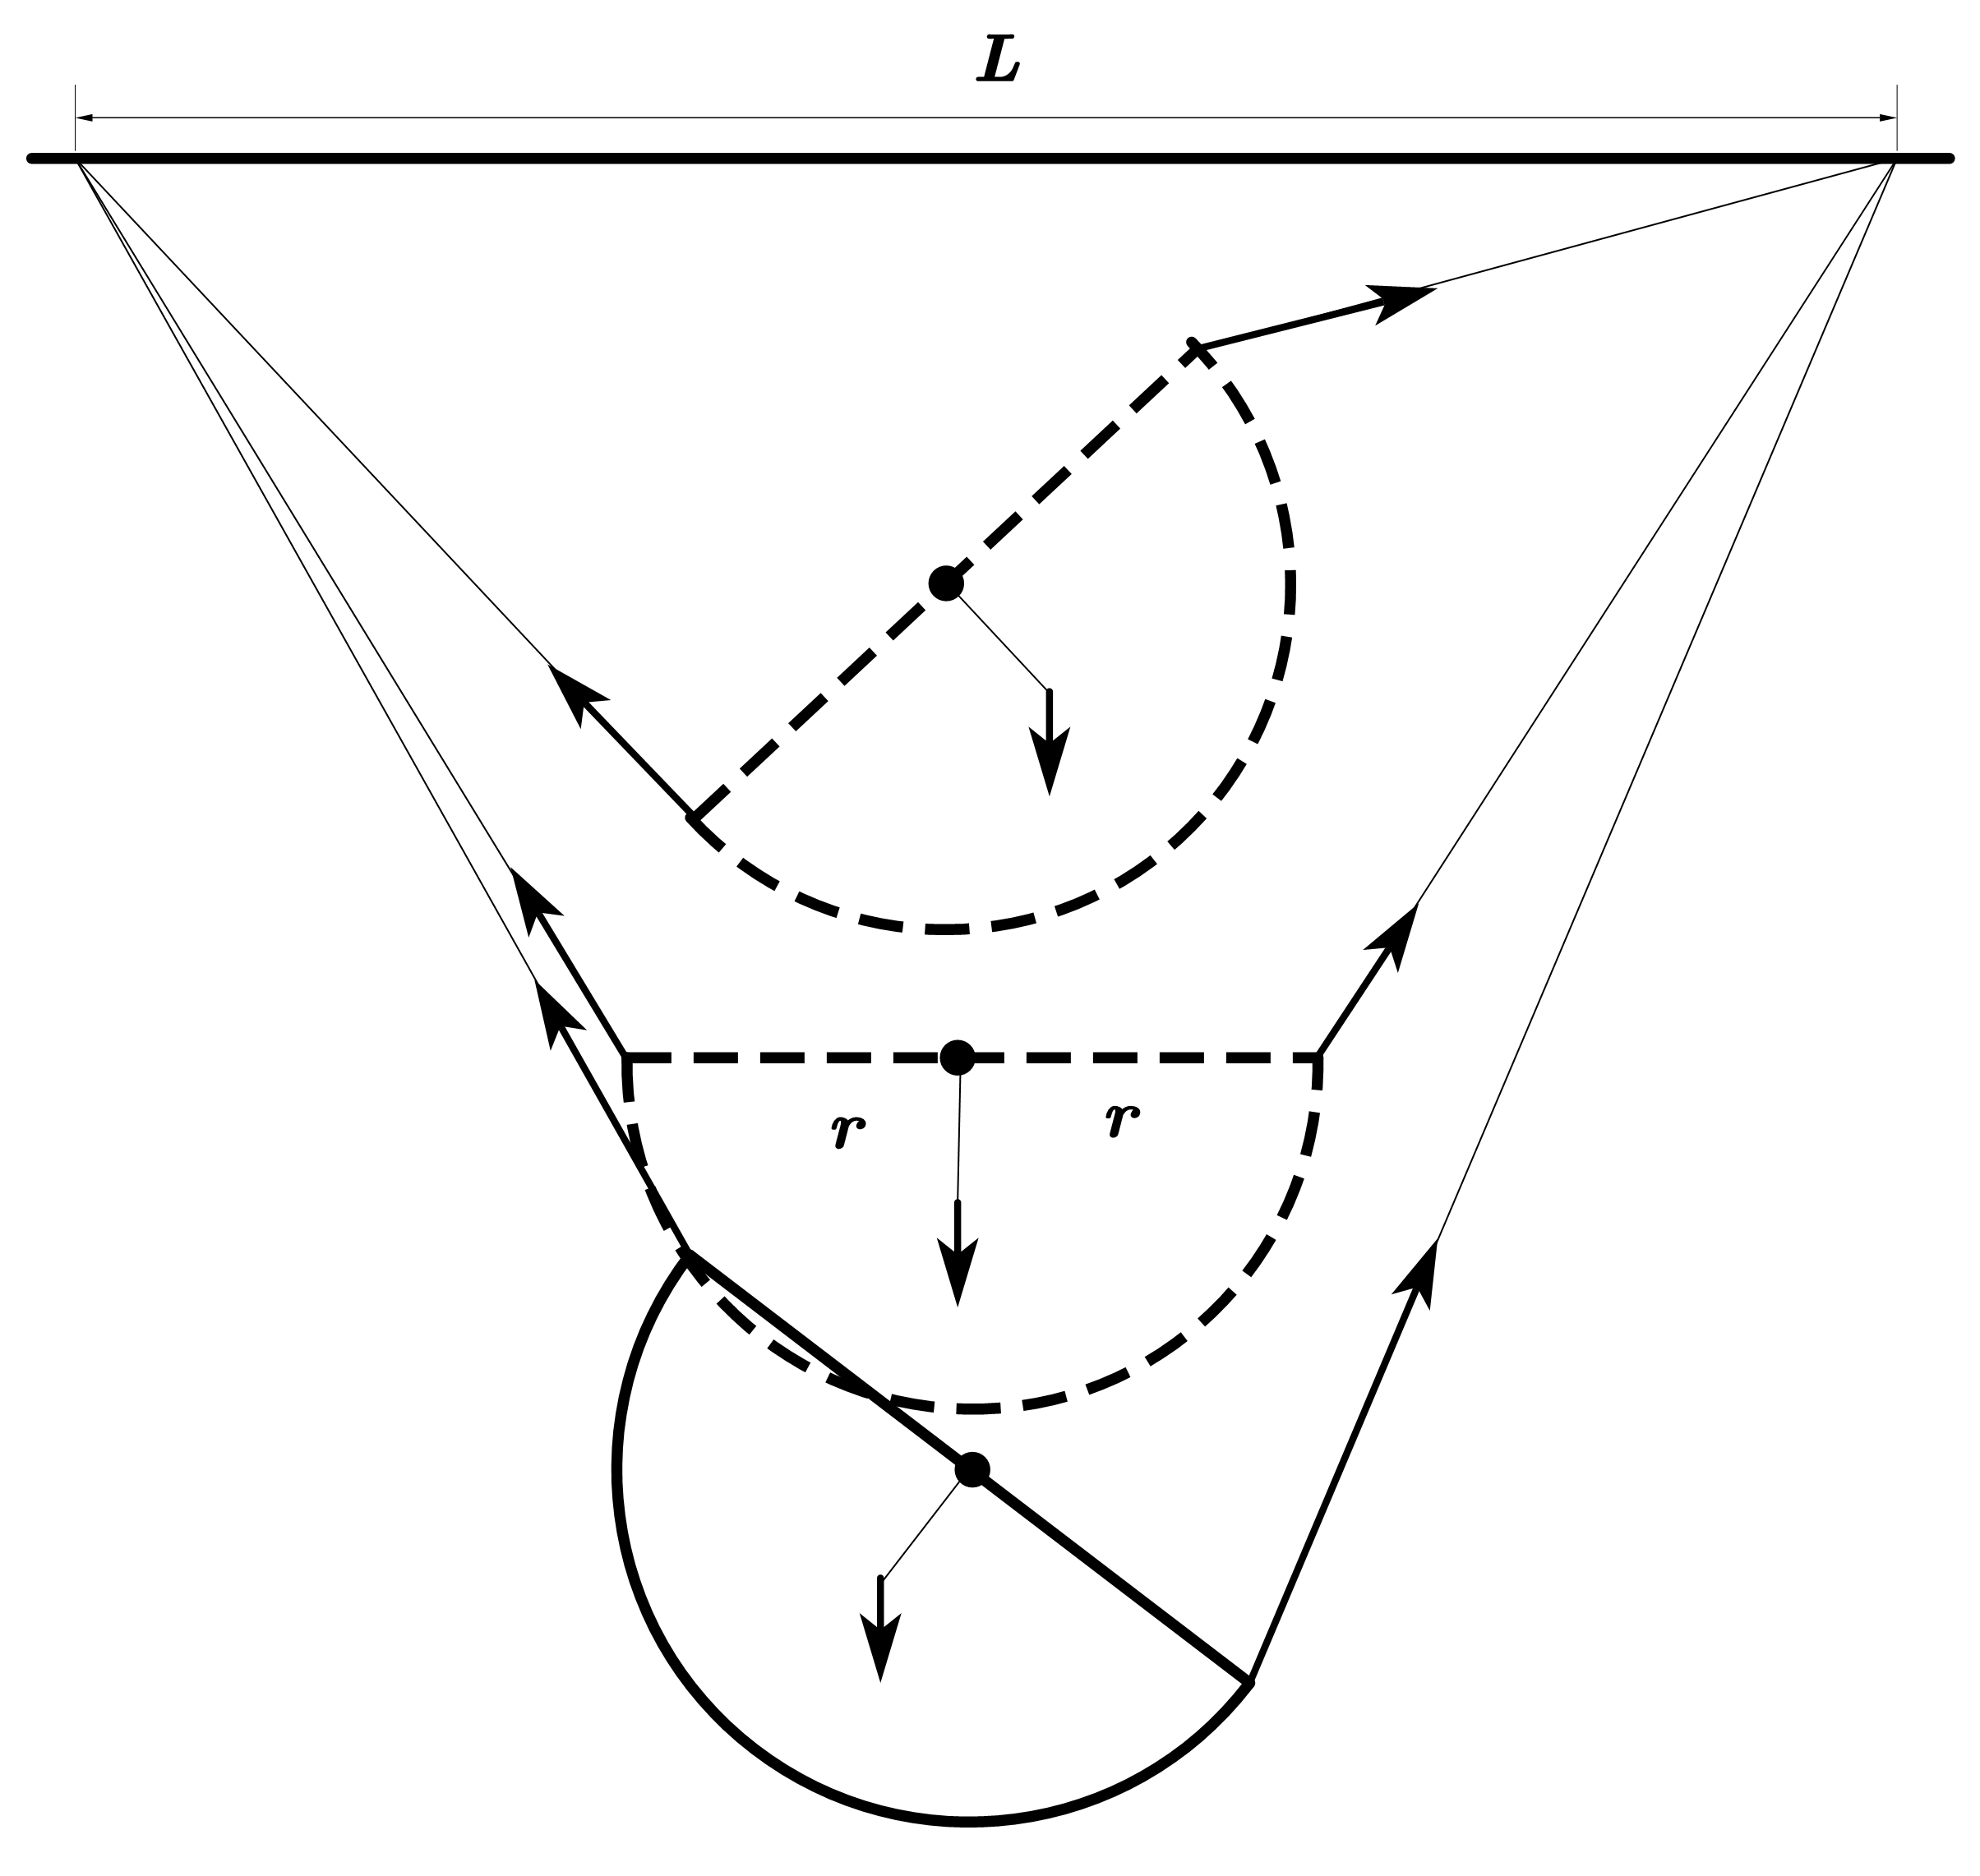
\includegraphics[height=0.3\textheight,width=0.9\textwidth]{问题3-2实际情况1}
		\caption{问题3-2\quad$\theta$角较大时实际变化情况示意图($L \neq 2r$)}
		\label{问题3-2实际情况1}
	\end{minipage}
\end{figure}

%	\begin{figure}
%	\centering
%	\begin{minipage}[c]{0.48\textwidth}
%		\centering
%		\includegraphics[height=0.2\textheight]{cat}
%		\subcaption{一只猫}
%	\end{minipage}
%	\begin{minipage}[c]{0.48\textwidth}
%		\centering
%		\includegraphics[height=0.2\textheight]{smokeblk}
%		\subcaption{电路图}
%	\end{minipage}
%	\caption{多图并排示例}
%\end{figure}

	 	\begin{figure}[H]
	\centering
	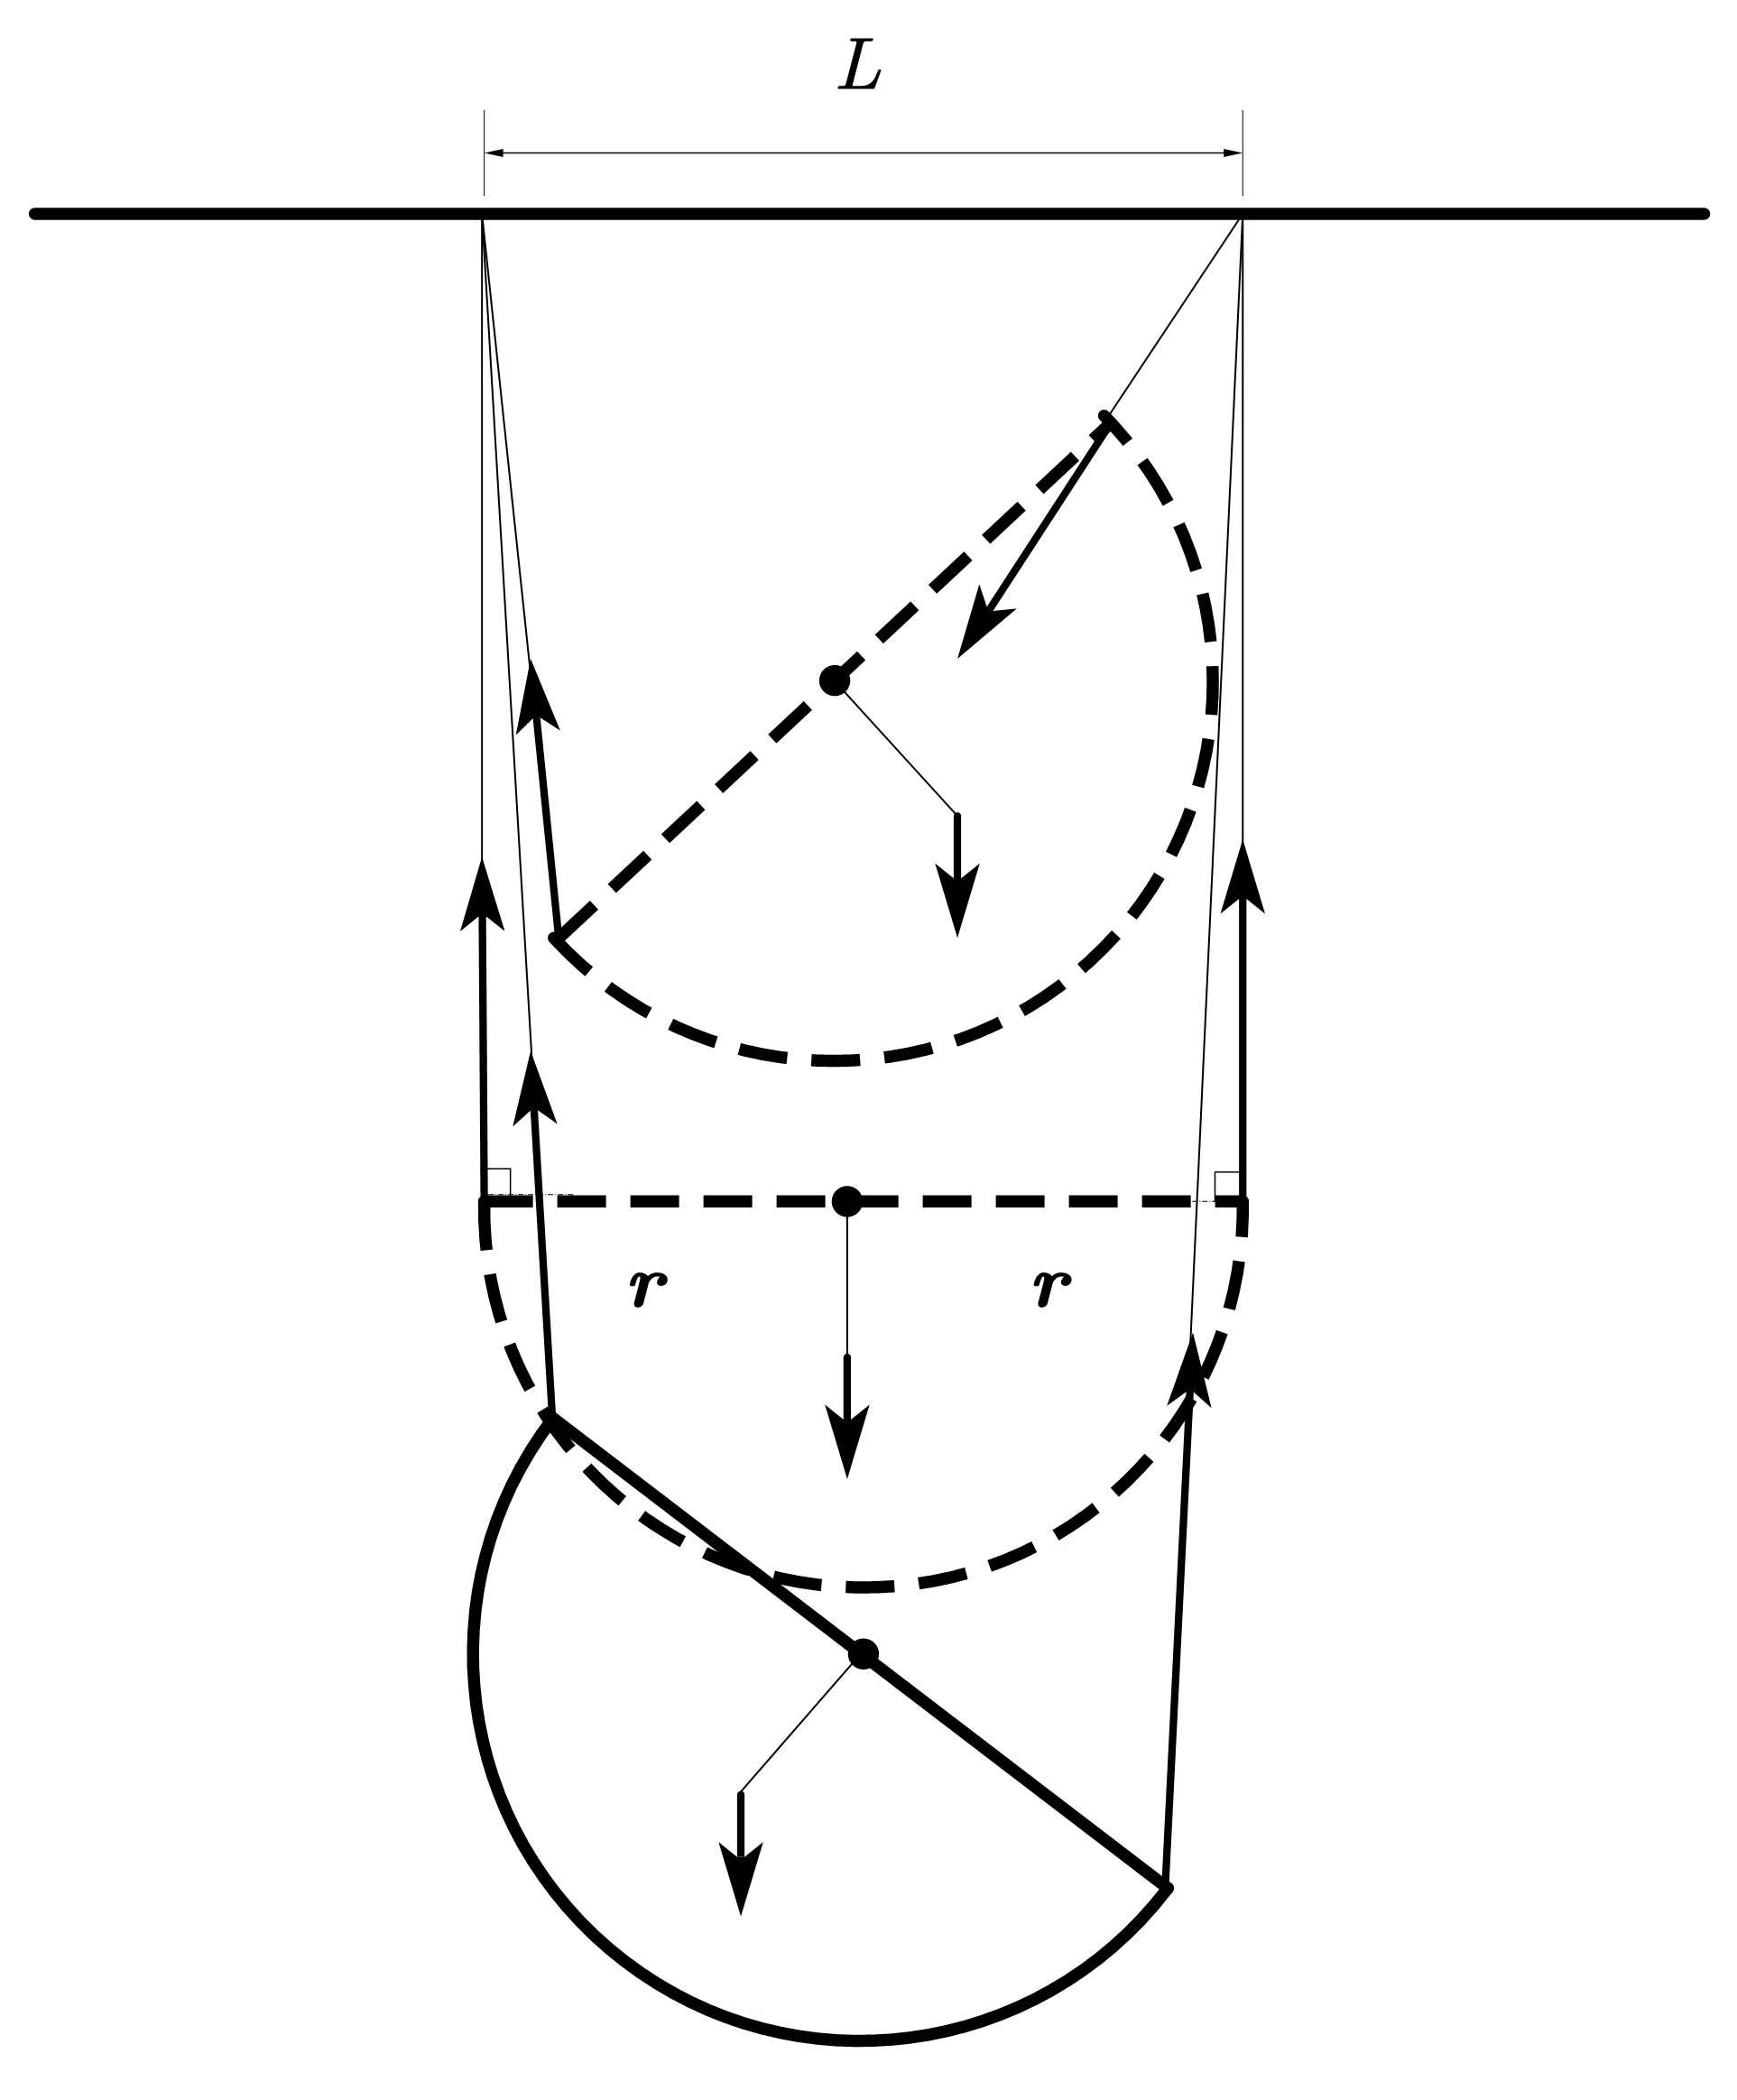
\includegraphics[height=0.3\textheight,]{问题3-2实际情况2}
	\caption{问题3-2 \quad$\theta$角较大时实际变化情况示意图($L = 2r$)}
	\label{问题3-2实际情况2}
\end{figure}

单独考虑竖直方向的运动,当$\theta_0$较大,半圆形薄片可看作质点,作出两种情况下的示意图:
	 	\begin{figure}[H]
	\centering
	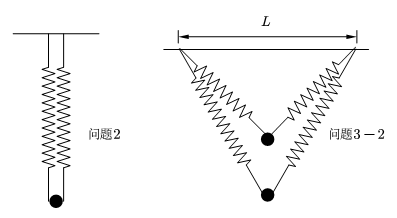
\includegraphics[width=0.7\textwidth]{实际情况简化}
	\caption{只考虑竖直方向运动的简化模型}
	\label{实际情况简化}
\end{figure}

对于问题二,竖直方向的运动为简谐运动,两弹簧并联的等效劲度系数为$2k$,运动周期为:
\begin{equation}\label{ydzq}
	T_{\text{竖直}}=2 \pi \sqrt{\frac{m}{2k}}=\frac{2\pi}{\sqrt{\frac{2k}{m}}}
\end{equation}
假设问题二模型中由式(\ref{czq22})
	\begin{equation}\label{czq22}
\left\{\begin{array}{l}
\theta^{\prime \prime}=-\frac{8g}{3 \pi r} \sin \theta-\frac{4 k}{m} \sin \theta \cos \theta \\
\theta(0)=\theta_{0} \quad \theta^{\prime}(0)=0
\end{array}\right.
\end{equation}

\noindent 通过数值法确定的转动周期为$	T_{\text{旋转}}$,与竖直运动周期式(\ref{ydzq})对比,实际的运动周期应该介于$T_{\text{旋转}}$和$T_{\text{竖直}}$之间。

对于问题3-2的简化模型,可做类似分析\upcite{caiShuangDanHuangZhenZiDeZhenDongFenXi2004,chenShuangDanHuangWenTiGuiLeiPouXi2018,halvorsenNewMethodEstimating1999,huangShuangDanHuangZhenZiZaiShuZhiFangXiangDeZiYouZhenDongYanJiu2014,liuShuangDanHuangZhiLiangXiTongZaiShuZhiFangXiangZhenDongDeShiYanYanJiu2013,wangJianXieJiLiXiaShuangDanHuangFeiXianXingNengLiangJingDeYouHua,weiShuangDanHuangXuanJiaXiTongTeXingFenXi2020a,zhangYuanTaiXingDanHuangZhiLiangDuiZhenDongZhouQiDeYingXiang2017,zhaoJiYuShuangDanHuangFuZaiDaoLiBaiMoXingDeBuTaiMoNi2021,zhaoShuangHengBiXuanJiaDongLiXueJianMoJiMoHuHuaMoKongZhiQiSheJi2021a}。其周期与$m,k,l,L$有关,为$\Phi(m,k,l,L)$,:假设由式(\ref{xs2})通过数值法确定的旋转周期为$	T_{\text{旋转}}$,与$T_{\text{竖直}}=\Phi(m,k,l,L)$ 对比
	\begin{equation}\label{xs2}
\left\{\begin{array}{l}
\begin{aligned}
&\theta^{\prime}=\omega \\
&\omega^{\prime}=f\left(x_{1}, x_{2}, \theta_{1}, \theta_{2}, \theta\right) \\
&\theta(0)=\theta_0,\omega(0)=0
\end{aligned}
\end{array}\right.
\end{equation}
实际的运动周期同样应该介于$T_{\text{旋转}}$和$T_{\text{竖直}}$之间。

	
	\section{模型的评价}
   本文对半圆形薄片系统建立受力方程、力矩方程、几何方程,通过数值法求解方程组得到了施加拉力后半圆形薄片的倾角。对问题二基于转动定理建立转动微分方程,通过几何关系建立变量之间的约束,利用ode45求解微分方程,求解得到的短期内角度时间演化很好地符合了实际。同时对$\theta \approx 0$的极限情况作了近似分析,求出其近似解析周期解。
   
   对于问题三,利用与前两问的相似性,添加了两个角度未知量,对应地建立方程组和微分代数方程,利用ode15或者迭代法+ode45求解,很好地描述了短期内的角度时间演化。
   
   问题一和问题3-1模型忽略了竖直方向运动,对模型作了简化,但也同时造成长期演化后,出现角度衰减的能量不守恒现象。因此只适用于$\theta$角较小的情形。最后,本文对$\theta$较大时的实际情况做了分析,综合考虑了转动和竖直方向运动,对竖直方向运动作出了简化的模型,描述了竖直运动的周期。得出了半圆形薄片的真实运动周期应该介于竖直运动周期和转动周期之间的结论。
   
   
   
   
	%\subsection{模型的推广}
	
	%参考文献
	%	\begin{thebibliography}{9}%宽度9
	%		\bibitem[1]{liuhaiyang2013latex}
	%		刘海洋.
	%		\newblock \LaTeX {}入门\allowbreak[J].
	%		\newblock 电子工业出版社, 北京, 2013.
	%		\bibitem[2]{mathematical-modeling}
	%		全国大学生数学建模竞赛论文格式规范 (2020 年 8 月 25 日修改).
	%		\bibitem{3} \url{https://www.latexstudio.net}
	%	\end{thebibliography}
	
	%\section{参考文献}
	%\addcontentsline{toc}{section}{参考文献}
	%\bibliographystyle{bib/gbt7714-2005}
	\bibliographystyle{gbt7714-numerical}
	%\bibliographystyle{unsrt}
	%\bibliographystyle{IEEEtran}
	\bibliography{bib/ref.bib}
	
	\newpage
	%附录
	\begin{appendices}
		\section{代码文件列表}
		% Table generated by Excel2LaTeX from sheet 'Sheet1'
		\begin{table}[htbp]
			\centering
			\begin{tabularx}{\textwidth}{@{}l *1{>{\centering\arraybackslash}X}@{}}
				\toprule[1.5pt]
				函数名   & 功能描述 \\
				\midrule
				config.m & 配置r,m,g,F,k等常数 \\
				question1.m & 问题一主程序 \\
				funq1.m & 问题一方程 \\
				question2.m & 问题二主程序 \\
				funq2.m & 问题二微分方程 \\
				plotT\_q2.m & 作T与r,m,k的关系图 \\
				question3\_1.m & 问题3-1主程序 \\
				funq3\_1.m & 问题3-1方程 \\
				question3\_2.m & 问题3-2主程序(ode15s) \\
				funq3\_2 & 问题3-2微分代数方程 \\
				question3\_2\_2.m & 问题3-2主程序(ode45) \\
				funq3\_2\_2.m & 问题3-2微分方程 \\
				funtest.m & 问题3-2代数方程 \\
				\bottomrule[1.5pt]
			\end{tabularx}%
			\label{tab:addlabel}%
		\end{table}%
		
		
		\section{代码}
		config.m:
		\lstinputlisting[language=matlab]{code/config.m} 
		question1.m 
		\lstinputlisting[language=matlab]{code/question1.m}  
		funq1.m
		\lstinputlisting[language=matlab]{code/funq1.m}  
		question2.m
		\lstinputlisting[language=matlab]{code/question2.m} 
		funq2.m 
		\lstinputlisting[language=matlab]{code/funq2.m} 
		plotT\_q2.m
		\lstinputlisting[language=matlab]{code/plotT_q2.m}
		question3\_1.m 
		\lstinputlisting[language=matlab]{code/question3_1.m} 
		funq3\_1.m 
		\lstinputlisting[language=matlab]{code/funq3_1.m} 
		question3\_2.m 
		\lstinputlisting[language=matlab]{code/question3_2.m}
		funq3\_2.m 
		\lstinputlisting[language=matlab]{code/funq3_2.m}
		question3\_2\_2.m 
		\lstinputlisting[language=matlab]{code/question3_2_2.m} 
		funq3\_2\_2.m
		\lstinputlisting[language=matlab]{code/funq3_2_2.m} 
		funtest.m
 		\lstinputlisting[language=matlab]{code/funtest.m} 
  
	\end{appendices}
	
\end{document} 